\documentclass[]{article}
\usepackage{lmodern}
\usepackage{amssymb,amsmath}
\usepackage{ifxetex,ifluatex}
\usepackage{fixltx2e} % provides \textsubscript
\ifnum 0\ifxetex 1\fi\ifluatex 1\fi=0 % if pdftex
  \usepackage[T1]{fontenc}
  \usepackage[utf8]{inputenc}
\else % if luatex or xelatex
  \ifxetex
    \usepackage{mathspec}
  \else
    \usepackage{fontspec}
  \fi
  \defaultfontfeatures{Ligatures=TeX,Scale=MatchLowercase}
\fi
% use upquote if available, for straight quotes in verbatim environments
\IfFileExists{upquote.sty}{\usepackage{upquote}}{}
% use microtype if available
\IfFileExists{microtype.sty}{%
\usepackage{microtype}
\UseMicrotypeSet[protrusion]{basicmath} % disable protrusion for tt fonts
}{}
\usepackage[margin=1in]{geometry}
\usepackage{hyperref}
\hypersetup{unicode=true,
            pdftitle={MSMB-Chapter2-Statistical Modelling},
            pdfauthor={Aleeza Gerstein},
            pdfborder={0 0 0},
            breaklinks=true}
\urlstyle{same}  % don't use monospace font for urls
\usepackage{color}
\usepackage{fancyvrb}
\newcommand{\VerbBar}{|}
\newcommand{\VERB}{\Verb[commandchars=\\\{\}]}
\DefineVerbatimEnvironment{Highlighting}{Verbatim}{commandchars=\\\{\}}
% Add ',fontsize=\small' for more characters per line
\usepackage{framed}
\definecolor{shadecolor}{RGB}{248,248,248}
\newenvironment{Shaded}{\begin{snugshade}}{\end{snugshade}}
\newcommand{\KeywordTok}[1]{\textcolor[rgb]{0.13,0.29,0.53}{\textbf{#1}}}
\newcommand{\DataTypeTok}[1]{\textcolor[rgb]{0.13,0.29,0.53}{#1}}
\newcommand{\DecValTok}[1]{\textcolor[rgb]{0.00,0.00,0.81}{#1}}
\newcommand{\BaseNTok}[1]{\textcolor[rgb]{0.00,0.00,0.81}{#1}}
\newcommand{\FloatTok}[1]{\textcolor[rgb]{0.00,0.00,0.81}{#1}}
\newcommand{\ConstantTok}[1]{\textcolor[rgb]{0.00,0.00,0.00}{#1}}
\newcommand{\CharTok}[1]{\textcolor[rgb]{0.31,0.60,0.02}{#1}}
\newcommand{\SpecialCharTok}[1]{\textcolor[rgb]{0.00,0.00,0.00}{#1}}
\newcommand{\StringTok}[1]{\textcolor[rgb]{0.31,0.60,0.02}{#1}}
\newcommand{\VerbatimStringTok}[1]{\textcolor[rgb]{0.31,0.60,0.02}{#1}}
\newcommand{\SpecialStringTok}[1]{\textcolor[rgb]{0.31,0.60,0.02}{#1}}
\newcommand{\ImportTok}[1]{#1}
\newcommand{\CommentTok}[1]{\textcolor[rgb]{0.56,0.35,0.01}{\textit{#1}}}
\newcommand{\DocumentationTok}[1]{\textcolor[rgb]{0.56,0.35,0.01}{\textbf{\textit{#1}}}}
\newcommand{\AnnotationTok}[1]{\textcolor[rgb]{0.56,0.35,0.01}{\textbf{\textit{#1}}}}
\newcommand{\CommentVarTok}[1]{\textcolor[rgb]{0.56,0.35,0.01}{\textbf{\textit{#1}}}}
\newcommand{\OtherTok}[1]{\textcolor[rgb]{0.56,0.35,0.01}{#1}}
\newcommand{\FunctionTok}[1]{\textcolor[rgb]{0.00,0.00,0.00}{#1}}
\newcommand{\VariableTok}[1]{\textcolor[rgb]{0.00,0.00,0.00}{#1}}
\newcommand{\ControlFlowTok}[1]{\textcolor[rgb]{0.13,0.29,0.53}{\textbf{#1}}}
\newcommand{\OperatorTok}[1]{\textcolor[rgb]{0.81,0.36,0.00}{\textbf{#1}}}
\newcommand{\BuiltInTok}[1]{#1}
\newcommand{\ExtensionTok}[1]{#1}
\newcommand{\PreprocessorTok}[1]{\textcolor[rgb]{0.56,0.35,0.01}{\textit{#1}}}
\newcommand{\AttributeTok}[1]{\textcolor[rgb]{0.77,0.63,0.00}{#1}}
\newcommand{\RegionMarkerTok}[1]{#1}
\newcommand{\InformationTok}[1]{\textcolor[rgb]{0.56,0.35,0.01}{\textbf{\textit{#1}}}}
\newcommand{\WarningTok}[1]{\textcolor[rgb]{0.56,0.35,0.01}{\textbf{\textit{#1}}}}
\newcommand{\AlertTok}[1]{\textcolor[rgb]{0.94,0.16,0.16}{#1}}
\newcommand{\ErrorTok}[1]{\textcolor[rgb]{0.64,0.00,0.00}{\textbf{#1}}}
\newcommand{\NormalTok}[1]{#1}
\usepackage{graphicx,grffile}
\makeatletter
\def\maxwidth{\ifdim\Gin@nat@width>\linewidth\linewidth\else\Gin@nat@width\fi}
\def\maxheight{\ifdim\Gin@nat@height>\textheight\textheight\else\Gin@nat@height\fi}
\makeatother
% Scale images if necessary, so that they will not overflow the page
% margins by default, and it is still possible to overwrite the defaults
% using explicit options in \includegraphics[width, height, ...]{}
\setkeys{Gin}{width=\maxwidth,height=\maxheight,keepaspectratio}
\IfFileExists{parskip.sty}{%
\usepackage{parskip}
}{% else
\setlength{\parindent}{0pt}
\setlength{\parskip}{6pt plus 2pt minus 1pt}
}
\setlength{\emergencystretch}{3em}  % prevent overfull lines
\providecommand{\tightlist}{%
  \setlength{\itemsep}{0pt}\setlength{\parskip}{0pt}}
\setcounter{secnumdepth}{0}
% Redefines (sub)paragraphs to behave more like sections
\ifx\paragraph\undefined\else
\let\oldparagraph\paragraph
\renewcommand{\paragraph}[1]{\oldparagraph{#1}\mbox{}}
\fi
\ifx\subparagraph\undefined\else
\let\oldsubparagraph\subparagraph
\renewcommand{\subparagraph}[1]{\oldsubparagraph{#1}\mbox{}}
\fi

%%% Use protect on footnotes to avoid problems with footnotes in titles
\let\rmarkdownfootnote\footnote%
\def\footnote{\protect\rmarkdownfootnote}

%%% Change title format to be more compact
\usepackage{titling}

% Create subtitle command for use in maketitle
\providecommand{\subtitle}[1]{
  \posttitle{
    \begin{center}\large#1\end{center}
    }
}

\setlength{\droptitle}{-2em}

  \title{MSMB-Chapter2-Statistical Modelling}
    \pretitle{\vspace{\droptitle}\centering\huge}
  \posttitle{\par}
    \author{Aleeza Gerstein}
    \preauthor{\centering\large\emph}
  \postauthor{\par}
      \predate{\centering\large\emph}
  \postdate{\par}
    \date{2019-09-16}

\usepackage{color}
\usepackage{mathtools}

\begin{document}
\maketitle

\section{Chapter 2: Statistical
Modeling}\label{chapter-2-statistical-modeling}

\subsection{A simple example of statistical
modelling}\label{a-simple-example-of-statistical-modelling}

\begin{Shaded}
\begin{Highlighting}[]
\KeywordTok{load}\NormalTok{(}\KeywordTok{url}\NormalTok{(}\StringTok{"http://bios221.stanford.edu/data/e100.RData"}\NormalTok{))}
\NormalTok{e99 =}\StringTok{ }\NormalTok{e100[}\OperatorTok{-}\KeywordTok{which.max}\NormalTok{(e100)]}
\KeywordTok{barplot}\NormalTok{(}\KeywordTok{table}\NormalTok{(e99), }\DataTypeTok{space =} \FloatTok{0.8}\NormalTok{, }\DataTypeTok{col =} \StringTok{"chartreuse4"}\NormalTok{)}
\end{Highlighting}
\end{Shaded}

\begin{figure}
\centering
\includegraphics{MSMB-Chapter2_files/figure-latex/barplot_pois-1.pdf}
\caption{The observed distribution of the epitope data without the
outlier.}
\end{figure}

\begin{Shaded}
\begin{Highlighting}[]
\KeywordTok{library}\NormalTok{(}\StringTok{"vcd"}\NormalTok{)}
\end{Highlighting}
\end{Shaded}

\begin{verbatim}
## Loading required package: grid
\end{verbatim}

\begin{Shaded}
\begin{Highlighting}[]
\NormalTok{gf1 =}\StringTok{ }\KeywordTok{goodfit}\NormalTok{(e99, }\StringTok{"poisson"}\NormalTok{)}
\KeywordTok{rootogram}\NormalTok{(gf1, }\DataTypeTok{xlab =} \StringTok{""}\NormalTok{, }\DataTypeTok{rect_gp =} \KeywordTok{gpar}\NormalTok{(}\DataTypeTok{fill =} \StringTok{"chartreuse4"}\NormalTok{))}
\end{Highlighting}
\end{Shaded}

\begin{figure}
\centering
\includegraphics{MSMB-Chapter2_files/figure-latex/stat-rooto-1.pdf}
\caption{Rootogram showing the square root of the theoretical values as
red dots and the square root of the observed frequencies as drop down
rectangles. (We'll see a bit below how the \texttt{goodfit} function
decided which \(\lambda\) to use.)}
\end{figure}

\textcolor{blue}{We will learn later what this is?}

\begin{center}\rule{0.5\linewidth}{\linethickness}\end{center}

\textcolor{red}{Question 1: To calibrate what such a plot looks like a known poisson variable, use `rpois` and $\lambda$ = 0.05 to generate 100 Poisson distributed numbers and draw their rootogram}

\begin{Shaded}
\begin{Highlighting}[]
\NormalTok{pv <-}\StringTok{ }\KeywordTok{rpois}\NormalTok{(}\DecValTok{100}\NormalTok{, }\FloatTok{0.05}\NormalTok{)}
\NormalTok{gf_pv =}\StringTok{ }\KeywordTok{goodfit}\NormalTok{(pv, }\StringTok{"poisson"}\NormalTok{)}
\KeywordTok{rootogram}\NormalTok{(gf_pv, }\DataTypeTok{xlab =} \StringTok{""}\NormalTok{, }\DataTypeTok{rect_gp =} \KeywordTok{gpar}\NormalTok{(}\DataTypeTok{fill =} \StringTok{"chartreuse4"}\NormalTok{))}
\end{Highlighting}
\end{Shaded}

\includegraphics{MSMB-Chapter2_files/figure-latex/Q1-1.pdf}

\begin{center}\rule{0.5\linewidth}{\linethickness}\end{center}

\begin{center}\rule{0.5\linewidth}{\linethickness}\end{center}

\textcolor{red}{Question 2: Repeat the simulation with different values of $\lambda$. Can you find one that gives cout close to the observed count by trial and error?}

\begin{Shaded}
\begin{Highlighting}[]
\KeywordTok{table}\NormalTok{(e100)}
\end{Highlighting}
\end{Shaded}

\begin{verbatim}
## e100
##  0  1  2  7 
## 58 34  7  1
\end{verbatim}

\begin{Shaded}
\begin{Highlighting}[]
\NormalTok{pv0.}\DecValTok{5}\NormalTok{ <-}\StringTok{ }\KeywordTok{rpois}\NormalTok{(}\DecValTok{100}\NormalTok{, }\FloatTok{0.5}\NormalTok{)}
\KeywordTok{table}\NormalTok{(pv0.}\DecValTok{5}\NormalTok{)}
\end{Highlighting}
\end{Shaded}

\begin{verbatim}
## pv0.5
##  0  1  2  3 
## 62 31  6  1
\end{verbatim}

\begin{center}\rule{0.5\linewidth}{\linethickness}\end{center}

\begin{Shaded}
\begin{Highlighting}[]
\NormalTok{loglikelihood  =}\StringTok{  }\ControlFlowTok{function}\NormalTok{(lambda, }\DataTypeTok{data =}\NormalTok{ e100) \{}
  \KeywordTok{sum}\NormalTok{(}\KeywordTok{log}\NormalTok{(}\KeywordTok{dpois}\NormalTok{(data, lambda)))}
\NormalTok{\}}
\end{Highlighting}
\end{Shaded}

\begin{Shaded}
\begin{Highlighting}[]
\NormalTok{lambdas =}\StringTok{ }\KeywordTok{seq}\NormalTok{(}\FloatTok{0.05}\NormalTok{, }\FloatTok{0.95}\NormalTok{, }\DataTypeTok{length =} \DecValTok{100}\NormalTok{)}
\NormalTok{loglik =}\StringTok{ }\KeywordTok{vapply}\NormalTok{(lambdas, loglikelihood, }\KeywordTok{numeric}\NormalTok{(}\DecValTok{1}\NormalTok{))}
\CommentTok{#this is the same as}
\CommentTok{#loglik = sapply(lambdas, loglikelihood)}
\KeywordTok{plot}\NormalTok{(lambdas, loglik, }\DataTypeTok{type =} \StringTok{"l"}\NormalTok{, }\DataTypeTok{col =} \StringTok{"red"}\NormalTok{, }\DataTypeTok{ylab =} \StringTok{""}\NormalTok{, }\DataTypeTok{lwd =} \DecValTok{2}\NormalTok{,}
     \DataTypeTok{xlab =} \KeywordTok{expression}\NormalTok{(lambda))}
\NormalTok{m0 =}\StringTok{ }\KeywordTok{mean}\NormalTok{(e100)}
\KeywordTok{abline}\NormalTok{(}\DataTypeTok{v =}\NormalTok{ m0, }\DataTypeTok{col =} \StringTok{"blue"}\NormalTok{, }\DataTypeTok{lwd =} \DecValTok{2}\NormalTok{)}
\KeywordTok{abline}\NormalTok{(}\DataTypeTok{h =} \KeywordTok{loglikelihood}\NormalTok{(m0), }\DataTypeTok{col =} \StringTok{"purple"}\NormalTok{, }\DataTypeTok{lwd =} \DecValTok{2}\NormalTok{)}
\end{Highlighting}
\end{Shaded}

\begin{figure}
\centering
\includegraphics{MSMB-Chapter2_files/figure-latex/chap2-r-poislikel-1-1.pdf}
\caption{The red curve is the log-likelihood function. The vertical line
shows the value of \texttt{m} (the mean) and the horizontal line the
log-likelihood of \texttt{m}. It looks like \texttt{m} maximizes the
likelihood.}
\end{figure}

\begin{Shaded}
\begin{Highlighting}[]
\NormalTok{m0}
\end{Highlighting}
\end{Shaded}

\begin{verbatim}
## [1] 0.55
\end{verbatim}

\begin{Shaded}
\begin{Highlighting}[]
\NormalTok{gf  =}\StringTok{  }\KeywordTok{goodfit}\NormalTok{(e100, }\StringTok{"poisson"}\NormalTok{)}
\KeywordTok{names}\NormalTok{(gf)}
\end{Highlighting}
\end{Shaded}

\begin{verbatim}
## [1] "observed" "count"    "fitted"   "type"     "method"   "df"      
## [7] "par"
\end{verbatim}

\begin{Shaded}
\begin{Highlighting}[]
\NormalTok{gf}\OperatorTok{$}\NormalTok{par}
\end{Highlighting}
\end{Shaded}

\begin{verbatim}
## $lambda
## [1] 0.55
\end{verbatim}

\begin{Shaded}
\begin{Highlighting}[]
\NormalTok{cb  =}\StringTok{  }\KeywordTok{c}\NormalTok{(}\KeywordTok{rep}\NormalTok{(}\DecValTok{0}\NormalTok{, }\DecValTok{110}\NormalTok{), }\KeywordTok{rep}\NormalTok{(}\DecValTok{1}\NormalTok{, }\DecValTok{10}\NormalTok{))}
\KeywordTok{table}\NormalTok{(cb)}
\end{Highlighting}
\end{Shaded}

\begin{verbatim}
## cb
##   0   1 
## 110  10
\end{verbatim}

\begin{Shaded}
\begin{Highlighting}[]
\NormalTok{probs  =}\StringTok{  }\KeywordTok{seq}\NormalTok{(}\DecValTok{0}\NormalTok{, }\FloatTok{0.3}\NormalTok{, }\DataTypeTok{by =} \FloatTok{0.005}\NormalTok{)}
\NormalTok{likelihood =}\StringTok{ }\KeywordTok{dbinom}\NormalTok{(}\KeywordTok{sum}\NormalTok{(cb), }\DataTypeTok{prob =}\NormalTok{ probs, }\DataTypeTok{size =} \KeywordTok{length}\NormalTok{(cb))}
\KeywordTok{plot}\NormalTok{(probs, likelihood, }\DataTypeTok{pch =} \DecValTok{16}\NormalTok{, }\DataTypeTok{xlab =} \StringTok{"probability of success"}\NormalTok{,}
     \DataTypeTok{ylab =} \StringTok{"likelihood"}\NormalTok{, }\DataTypeTok{cex=}\FloatTok{0.6}\NormalTok{)}
\end{Highlighting}
\end{Shaded}

\begin{figure}
\centering
\includegraphics{MSMB-Chapter2_files/figure-latex/likely1-1.pdf}
\caption{Plot of the likelihood as a function of the probabilities. The
likelihood is a function on \([0, 1]\); here we have zoomed into the
range of \([(ref:likely1-1), (ref:likely1-2)]\), as the likelihood is
practically zero for larger values of \(p\).}
\end{figure}

\begin{Shaded}
\begin{Highlighting}[]
\NormalTok{probs[}\KeywordTok{which.max}\NormalTok{(likelihood)]}
\end{Highlighting}
\end{Shaded}

\begin{verbatim}
## [1] 0.085
\end{verbatim}

\begin{Shaded}
\begin{Highlighting}[]
\KeywordTok{stopifnot}\NormalTok{(}\KeywordTok{abs}\NormalTok{(probs[}\KeywordTok{which.max}\NormalTok{(likelihood)]}\OperatorTok{-}\DecValTok{1}\OperatorTok{/}\DecValTok{12}\NormalTok{) }\OperatorTok{<}\StringTok{ }\KeywordTok{diff}\NormalTok{(probs[}\DecValTok{1}\OperatorTok{:}\DecValTok{2}\NormalTok{]))}
\end{Highlighting}
\end{Shaded}

\begin{Shaded}
\begin{Highlighting}[]
\NormalTok{loglikelihood =}\StringTok{ }\ControlFlowTok{function}\NormalTok{(theta, }\DataTypeTok{n =} \DecValTok{300}\NormalTok{, }\DataTypeTok{k =} \DecValTok{40}\NormalTok{) \{}
  \DecValTok{115} \OperatorTok{+}\StringTok{ }\NormalTok{k }\OperatorTok{*}\StringTok{ }\KeywordTok{log}\NormalTok{(theta) }\OperatorTok{+}\StringTok{ }\NormalTok{(n }\OperatorTok{-}\StringTok{ }\NormalTok{k) }\OperatorTok{*}\StringTok{ }\KeywordTok{log}\NormalTok{(}\DecValTok{1} \OperatorTok{-}\StringTok{ }\NormalTok{theta)}
\NormalTok{\}}
\end{Highlighting}
\end{Shaded}

\begin{Shaded}
\begin{Highlighting}[]
\NormalTok{thetas =}\StringTok{ }\KeywordTok{seq}\NormalTok{(}\DecValTok{0}\NormalTok{, }\DecValTok{1}\NormalTok{, }\DataTypeTok{by =} \FloatTok{0.001}\NormalTok{)}
\KeywordTok{plot}\NormalTok{(thetas, }\KeywordTok{loglikelihood}\NormalTok{(thetas), }\DataTypeTok{xlab =} \KeywordTok{expression}\NormalTok{(theta),}
     \DataTypeTok{ylab =} \KeywordTok{expression}\NormalTok{(}\KeywordTok{paste}\NormalTok{(}\StringTok{"log f("}\NormalTok{, theta, }\StringTok{" | y)"}\NormalTok{)),}\DataTypeTok{type =} \StringTok{"l"}\NormalTok{)}
\end{Highlighting}
\end{Shaded}

\begin{figure}
\centering
\includegraphics{MSMB-Chapter2_files/figure-latex/chap2-r-loglikelihood-1-1.pdf}
\caption{Plot of the log likelihood function for \(n=300\) and
\(y=40\).}
\end{figure}

\begin{Shaded}
\begin{Highlighting}[]
\KeywordTok{library}\NormalTok{(}\StringTok{"Biostrings"}\NormalTok{)}
\end{Highlighting}
\end{Shaded}

\begin{verbatim}
## Loading required package: BiocGenerics
\end{verbatim}

\begin{verbatim}
## Loading required package: parallel
\end{verbatim}

\begin{verbatim}
## 
## Attaching package: 'BiocGenerics'
\end{verbatim}

\begin{verbatim}
## The following objects are masked from 'package:parallel':
## 
##     clusterApply, clusterApplyLB, clusterCall, clusterEvalQ,
##     clusterExport, clusterMap, parApply, parCapply, parLapply,
##     parLapplyLB, parRapply, parSapply, parSapplyLB
\end{verbatim}

\begin{verbatim}
## The following objects are masked from 'package:stats':
## 
##     IQR, mad, sd, var, xtabs
\end{verbatim}

\begin{verbatim}
## The following objects are masked from 'package:base':
## 
##     anyDuplicated, append, as.data.frame, basename, cbind,
##     colnames, dirname, do.call, duplicated, eval, evalq, Filter,
##     Find, get, grep, grepl, intersect, is.unsorted, lapply, Map,
##     mapply, match, mget, order, paste, pmax, pmax.int, pmin,
##     pmin.int, Position, rank, rbind, Reduce, rownames, sapply,
##     setdiff, sort, table, tapply, union, unique, unsplit, which,
##     which.max, which.min
\end{verbatim}

\begin{verbatim}
## Loading required package: S4Vectors
\end{verbatim}

\begin{verbatim}
## Loading required package: stats4
\end{verbatim}

\begin{verbatim}
## 
## Attaching package: 'S4Vectors'
\end{verbatim}

\begin{verbatim}
## The following object is masked from 'package:base':
## 
##     expand.grid
\end{verbatim}

\begin{verbatim}
## Loading required package: IRanges
\end{verbatim}

\begin{verbatim}
## 
## Attaching package: 'IRanges'
\end{verbatim}

\begin{verbatim}
## The following object is masked from 'package:vcd':
## 
##     tile
\end{verbatim}

\begin{verbatim}
## Loading required package: XVector
\end{verbatim}

\begin{verbatim}
## 
## Attaching package: 'Biostrings'
\end{verbatim}

\begin{verbatim}
## The following object is masked from 'package:base':
## 
##     strsplit
\end{verbatim}

\begin{Shaded}
\begin{Highlighting}[]
\NormalTok{staph =}\StringTok{ }\KeywordTok{readDNAStringSet}\NormalTok{(}\StringTok{"http://bios221.stanford.edu/data/staphsequence.ffn.txt"}\NormalTok{, }\StringTok{"fasta"}\NormalTok{)}
\NormalTok{staph[}\DecValTok{1}\NormalTok{]}
\end{Highlighting}
\end{Shaded}

\begin{verbatim}
##   A DNAStringSet instance of length 1
##     width seq                                          names               
## [1]  1362 ATGTCGGAAAAAGAAATTTGG...AAGAAATAAGAAATGTATAA lcl|NC_002952.2_c...
\end{verbatim}

\begin{Shaded}
\begin{Highlighting}[]
\KeywordTok{letterFrequency}\NormalTok{(staph[[}\DecValTok{1}\NormalTok{]], }\DataTypeTok{letters =} \StringTok{"ACGT"}\NormalTok{, }\DataTypeTok{OR =} \DecValTok{0}\NormalTok{)}
\end{Highlighting}
\end{Shaded}

\begin{verbatim}
##   A   C   G   T 
## 522 219 229 392
\end{verbatim}

\begin{center}\rule{0.5\linewidth}{\linethickness}\end{center}

\textcolor{red}{Question 2.9: Following a similar procedure to Exercise 1.8, test whether the nucleotides are equally distributed across the four possibilities for this first gene.}

\begin{Shaded}
\begin{Highlighting}[]
\NormalTok{lf <-}\StringTok{ }\KeywordTok{letterFrequency}\NormalTok{(staph[[}\DecValTok{1}\NormalTok{]], }\DataTypeTok{letters =} \StringTok{"ACGT"}\NormalTok{, }\DataTypeTok{OR =} \DecValTok{0}\NormalTok{)}
\KeywordTok{t}\NormalTok{(}\KeywordTok{rmultinom}\NormalTok{(}\DecValTok{1}\NormalTok{, }\KeywordTok{sum}\NormalTok{(lf), }\DataTypeTok{p =} \KeywordTok{rep}\NormalTok{(}\DecValTok{1}\OperatorTok{/}\DecValTok{4}\NormalTok{, }\DecValTok{4}\NormalTok{)))}
\end{Highlighting}
\end{Shaded}

\begin{verbatim}
##      [,1] [,2] [,3] [,4]
## [1,]  360  342  323  337
\end{verbatim}

\begin{Shaded}
\begin{Highlighting}[]
\NormalTok{oestat <-}\StringTok{ }\ControlFlowTok{function}\NormalTok{(o, e) \{}
  \KeywordTok{sum}\NormalTok{((e}\OperatorTok{-}\NormalTok{o)}\OperatorTok{^}\DecValTok{2} \OperatorTok{/}\StringTok{ }\NormalTok{e)}
\NormalTok{\}}

\NormalTok{B =}\StringTok{ }\DecValTok{1000}
\NormalTok{n =}\StringTok{ }\KeywordTok{sum}\NormalTok{(lf)}
\NormalTok{expected =}\StringTok{ }\KeywordTok{rep}\NormalTok{(n }\OperatorTok{/}\StringTok{ }\DecValTok{4}\NormalTok{, }\DecValTok{4}\NormalTok{)}

\NormalTok{oenull <-}\StringTok{ }\KeywordTok{replicate}\NormalTok{(B,}
  \KeywordTok{oestat}\NormalTok{(}\DataTypeTok{e =}\NormalTok{ expected, }\DataTypeTok{o =} \KeywordTok{rmultinom}\NormalTok{(}\DecValTok{1}\NormalTok{, n, }\DataTypeTok{p =} \KeywordTok{rep}\NormalTok{(}\DecValTok{1}\OperatorTok{/}\DecValTok{4}\NormalTok{, }\DecValTok{4}\NormalTok{))))}
\KeywordTok{hist}\NormalTok{(oenull, }\DataTypeTok{breaks =} \DecValTok{100}\NormalTok{, }\DataTypeTok{col =} \StringTok{"skyblue"}\NormalTok{, }\DataTypeTok{main=}\StringTok{""}\NormalTok{)}
\end{Highlighting}
\end{Shaded}

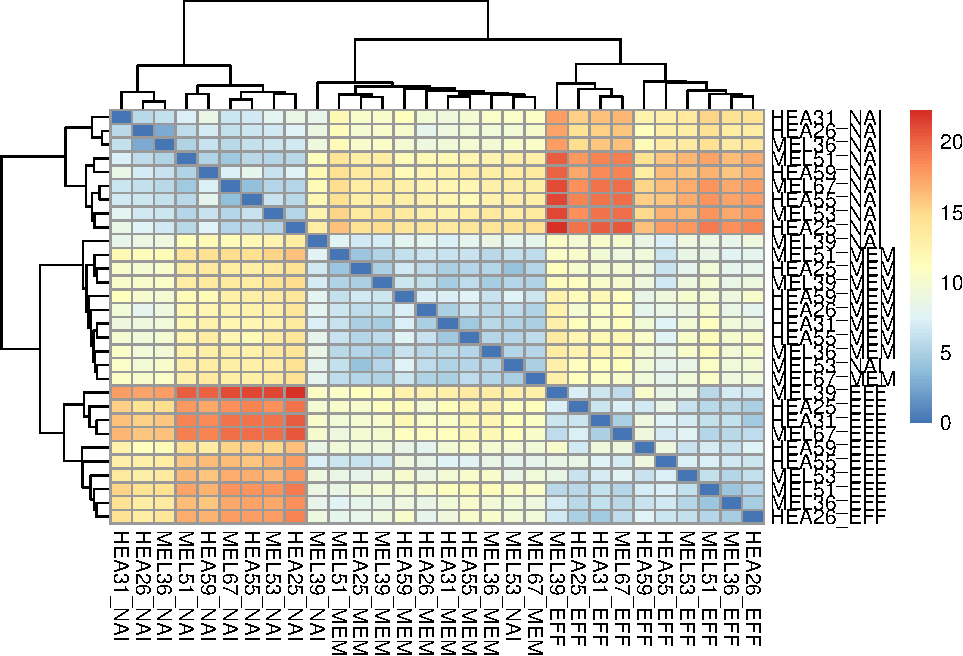
\includegraphics{MSMB-Chapter2_files/figure-latex/unnamed-chunk-6-1.pdf}

\begin{Shaded}
\begin{Highlighting}[]
\KeywordTok{oestat}\NormalTok{(}\DataTypeTok{e =}\NormalTok{ expected, }\DataTypeTok{o =} \KeywordTok{t}\NormalTok{(lf))}
\end{Highlighting}
\end{Shaded}

\begin{verbatim}
## [1] 184.4023
\end{verbatim}

\begin{Shaded}
\begin{Highlighting}[]
\KeywordTok{dmultinom}\NormalTok{(lf, }\DataTypeTok{prob =} \KeywordTok{rep}\NormalTok{(}\FloatTok{0.25}\NormalTok{, }\DecValTok{4}\NormalTok{))}
\end{Highlighting}
\end{Shaded}

\begin{verbatim}
## [1] 9.026662e-45
\end{verbatim}

\begin{center}\rule{0.5\linewidth}{\linethickness}\end{center}

\begin{Shaded}
\begin{Highlighting}[]
\NormalTok{letterFrq =}\StringTok{ }\KeywordTok{vapply}\NormalTok{(staph, letterFrequency, }\DataTypeTok{FUN.VALUE =} \KeywordTok{numeric}\NormalTok{(}\DecValTok{4}\NormalTok{),}
                   \DataTypeTok{letters =} \StringTok{"ACGT"}\NormalTok{, }\DataTypeTok{OR =} \DecValTok{0}\NormalTok{)}
\KeywordTok{colnames}\NormalTok{(letterFrq) =}\StringTok{ }\KeywordTok{paste0}\NormalTok{(}\StringTok{"gene"}\NormalTok{, }\KeywordTok{seq}\NormalTok{(}\DataTypeTok{along =}\NormalTok{ staph))}
\NormalTok{tab10 =}\StringTok{ }\NormalTok{letterFrq[, }\DecValTok{1}\OperatorTok{:}\DecValTok{10}\NormalTok{]}
\NormalTok{computeProportions =}\StringTok{ }\ControlFlowTok{function}\NormalTok{(x) \{ x}\OperatorTok{/}\KeywordTok{sum}\NormalTok{(x) \}}
\NormalTok{prop10 =}\StringTok{ }\KeywordTok{apply}\NormalTok{(tab10, }\DecValTok{2}\NormalTok{, computeProportions)}
\KeywordTok{round}\NormalTok{(prop10, }\DataTypeTok{digits =} \DecValTok{2}\NormalTok{)}
\end{Highlighting}
\end{Shaded}

\begin{verbatim}
##   gene1 gene2 gene3 gene4 gene5 gene6 gene7 gene8 gene9 gene10
## A  0.38  0.36  0.35  0.37  0.35  0.33  0.33  0.34  0.38   0.27
## C  0.16  0.16  0.13  0.15  0.15  0.15  0.16  0.16  0.14   0.16
## G  0.17  0.17  0.23  0.19  0.22  0.22  0.20  0.21  0.20   0.20
## T  0.29  0.31  0.30  0.29  0.27  0.30  0.30  0.29  0.28   0.36
\end{verbatim}

\begin{Shaded}
\begin{Highlighting}[]
\NormalTok{p0 =}\StringTok{ }\KeywordTok{rowMeans}\NormalTok{(prop10)}
\NormalTok{p0}
\end{Highlighting}
\end{Shaded}

\begin{verbatim}
##         A         C         G         T 
## 0.3470531 0.1518313 0.2011442 0.2999714
\end{verbatim}

\begin{Shaded}
\begin{Highlighting}[]
\NormalTok{cs =}\StringTok{ }\KeywordTok{colSums}\NormalTok{(tab10)}
\NormalTok{cs}
\end{Highlighting}
\end{Shaded}

\begin{verbatim}
##  gene1  gene2  gene3  gene4  gene5  gene6  gene7  gene8  gene9 gene10 
##   1362   1134    246   1113   1932   2661    831   1515   1287    696
\end{verbatim}

\begin{Shaded}
\begin{Highlighting}[]
\NormalTok{expectedtab10 =}\StringTok{ }\KeywordTok{outer}\NormalTok{(p0, cs, }\DataTypeTok{FUN =} \StringTok{"*"}\NormalTok{)}
\KeywordTok{round}\NormalTok{(expectedtab10)}
\end{Highlighting}
\end{Shaded}

\begin{verbatim}
##   gene1 gene2 gene3 gene4 gene5 gene6 gene7 gene8 gene9 gene10
## A   473   394    85   386   671   924   288   526   447    242
## C   207   172    37   169   293   404   126   230   195    106
## G   274   228    49   224   389   535   167   305   259    140
## T   409   340    74   334   580   798   249   454   386    209
\end{verbatim}

\begin{Shaded}
\begin{Highlighting}[]
\NormalTok{randomtab10 =}\StringTok{ }\KeywordTok{sapply}\NormalTok{(cs, }\ControlFlowTok{function}\NormalTok{(s) \{ }\KeywordTok{rmultinom}\NormalTok{(}\DecValTok{1}\NormalTok{, s, p0) \} )}
\KeywordTok{all}\NormalTok{(}\KeywordTok{colSums}\NormalTok{(randomtab10) }\OperatorTok{==}\StringTok{ }\NormalTok{cs)}
\end{Highlighting}
\end{Shaded}

\begin{verbatim}
## [1] TRUE
\end{verbatim}

\begin{Shaded}
\begin{Highlighting}[]
\NormalTok{stat =}\StringTok{ }\ControlFlowTok{function}\NormalTok{(obsvd, }\DataTypeTok{exptd =} \DecValTok{20} \OperatorTok{*}\StringTok{ }\NormalTok{pvec) \{}
  \KeywordTok{sum}\NormalTok{((obsvd }\OperatorTok{-}\StringTok{ }\NormalTok{exptd)}\OperatorTok{^}\DecValTok{2} \OperatorTok{/}\StringTok{ }\NormalTok{exptd)}
\NormalTok{\}}
\NormalTok{B =}\StringTok{ }\DecValTok{1000}
\NormalTok{simulstat =}\StringTok{ }\KeywordTok{replicate}\NormalTok{(B, \{}
\NormalTok{  randomtab10 =}\StringTok{ }\KeywordTok{sapply}\NormalTok{(cs, }\ControlFlowTok{function}\NormalTok{(s) \{ }\KeywordTok{rmultinom}\NormalTok{(}\DecValTok{1}\NormalTok{, s, p0) \})}
  \KeywordTok{stat}\NormalTok{(randomtab10, expectedtab10)}
\NormalTok{\})}
\NormalTok{S1 =}\StringTok{ }\KeywordTok{stat}\NormalTok{(tab10, expectedtab10)}
\KeywordTok{sum}\NormalTok{(simulstat }\OperatorTok{>=}\StringTok{ }\NormalTok{S1)}
\end{Highlighting}
\end{Shaded}

\begin{verbatim}
## [1] 0
\end{verbatim}

\begin{Shaded}
\begin{Highlighting}[]
\KeywordTok{hist}\NormalTok{(simulstat, }\DataTypeTok{col =} \StringTok{"lavender"}\NormalTok{, }\DataTypeTok{breaks =} \KeywordTok{seq}\NormalTok{(}\DecValTok{0}\NormalTok{, }\DecValTok{75}\NormalTok{, }\DataTypeTok{length.out=}\DecValTok{50}\NormalTok{))}
\KeywordTok{abline}\NormalTok{(}\DataTypeTok{v =}\NormalTok{ S1, }\DataTypeTok{col =} \StringTok{"red"}\NormalTok{)}
\KeywordTok{abline}\NormalTok{(}\DataTypeTok{v =} \KeywordTok{quantile}\NormalTok{(simulstat, }\DataTypeTok{probs =} \KeywordTok{c}\NormalTok{(}\FloatTok{0.95}\NormalTok{, }\FloatTok{0.99}\NormalTok{)),}
       \DataTypeTok{col =} \KeywordTok{c}\NormalTok{(}\StringTok{"darkgreen"}\NormalTok{, }\StringTok{"blue"}\NormalTok{), }\DataTypeTok{lty =} \DecValTok{2}\NormalTok{)}
\end{Highlighting}
\end{Shaded}

\begin{figure}
\centering
\includegraphics{MSMB-Chapter2_files/figure-latex/chap2-r-quant12-1-1.pdf}
\caption{Histogram of \texttt{simulstat}. The value of \texttt{S1} is
marked by the vertical red line, those of the 0.95 and 0.99 quantiles
(see next section) by the dotted lines.}
\end{figure}

\begin{Shaded}
\begin{Highlighting}[]
\NormalTok{qs =}\StringTok{ }\KeywordTok{ppoints}\NormalTok{(}\DecValTok{100}\NormalTok{)}
\KeywordTok{quantile}\NormalTok{(simulstat, qs)}
\KeywordTok{quantile}\NormalTok{(}\KeywordTok{qchisq}\NormalTok{(qs, }\DataTypeTok{df =} \DecValTok{30}\NormalTok{), qs)}
\end{Highlighting}
\end{Shaded}

\begin{Shaded}
\begin{Highlighting}[]
\KeywordTok{qqplot}\NormalTok{(}\KeywordTok{qchisq}\NormalTok{(}\KeywordTok{ppoints}\NormalTok{(B), }\DataTypeTok{df =} \DecValTok{30}\NormalTok{), simulstat, }\DataTypeTok{main =} \StringTok{""}\NormalTok{,}
       \DataTypeTok{xlab =} \KeywordTok{expression}\NormalTok{(chi[nu}\OperatorTok{==}\DecValTok{30}\NormalTok{]}\OperatorTok{^}\DecValTok{2}\NormalTok{), }\DataTypeTok{asp =} \DecValTok{1}\NormalTok{, }\DataTypeTok{cex =} \FloatTok{0.5}\NormalTok{, }\DataTypeTok{pch =} \DecValTok{16}\NormalTok{)}
\KeywordTok{abline}\NormalTok{(}\DataTypeTok{a =} \DecValTok{0}\NormalTok{, }\DataTypeTok{b =} \DecValTok{1}\NormalTok{, }\DataTypeTok{col =} \StringTok{"red"}\NormalTok{)}
\end{Highlighting}
\end{Shaded}

\begin{figure}
\centering
\includegraphics{MSMB-Chapter2_files/figure-latex/chap2-r-qqplot3-1-1.pdf}
\caption{Our simulated statistic's distribution compared to
\(\chi_{30}^2\) using a QQ-plot, which shows the theoretical
\textbf{quantiles} for the \(\chi^2_{30}\) distribution on the
horizontal axis and the sampled ones on the vertical axis.}
\end{figure}

\begin{Shaded}
\begin{Highlighting}[]
\DecValTok{1} \OperatorTok{-}\StringTok{ }\KeywordTok{pchisq}\NormalTok{(S1, }\DataTypeTok{df =} \DecValTok{30}\NormalTok{)}
\end{Highlighting}
\end{Shaded}

\begin{verbatim}
## [1] 4.74342e-05
\end{verbatim}

\begin{Shaded}
\begin{Highlighting}[]
\KeywordTok{load}\NormalTok{(}\KeywordTok{url}\NormalTok{(}\StringTok{"http://bios221.stanford.edu/data/ChargaffTable.RData"}\NormalTok{))}
\NormalTok{ChargaffTable}
\end{Highlighting}
\end{Shaded}

\begin{verbatim}
##                  A    T    C    G
## Human-Thymus  30.9 29.4 19.9 19.8
## Mycobac.Tuber 15.1 14.6 34.9 35.4
## Rat-          28.8 29.2 20.5 21.5
## Sheep-liver   29.3 29.3 20.5 20.7
## Sea Urchin    32.8 32.1 17.7 17.3
## Wheat         27.3 27.1 22.7 22.8
## Yeast         31.3 32.9 18.7 17.1
## E.coli        24.7 23.6 26.0 25.7
\end{verbatim}

\begin{figure}
\centering
\includegraphics{MSMB-Chapter2_files/figure-latex/ChargaffBars-1.pdf}
\caption{Barplots for the different rows in \texttt{ChargaffTable}. Can
you spot the pattern?}
\end{figure}

\begin{Shaded}
\begin{Highlighting}[]
\NormalTok{statChf =}\StringTok{ }\ControlFlowTok{function}\NormalTok{(x)\{}
  \KeywordTok{sum}\NormalTok{((x[, }\StringTok{"C"}\NormalTok{] }\OperatorTok{-}\StringTok{ }\NormalTok{x[, }\StringTok{"G"}\NormalTok{])}\OperatorTok{^}\DecValTok{2} \OperatorTok{+}\StringTok{ }\NormalTok{(x[, }\StringTok{"A"}\NormalTok{] }\OperatorTok{-}\StringTok{ }\NormalTok{x[, }\StringTok{"T"}\NormalTok{])}\OperatorTok{^}\DecValTok{2}\NormalTok{)}
\NormalTok{\}}
\NormalTok{chfstat =}\StringTok{ }\KeywordTok{statChf}\NormalTok{(ChargaffTable)}
\NormalTok{permstat =}\StringTok{ }\KeywordTok{replicate}\NormalTok{(}\DecValTok{100000}\NormalTok{, \{}
\NormalTok{  permuted =}\StringTok{ }\KeywordTok{t}\NormalTok{(}\KeywordTok{apply}\NormalTok{(ChargaffTable, }\DecValTok{1}\NormalTok{, sample))}
  \KeywordTok{colnames}\NormalTok{(permuted) =}\StringTok{ }\KeywordTok{colnames}\NormalTok{(ChargaffTable)}
  \KeywordTok{statChf}\NormalTok{(permuted)}
\NormalTok{\})}
\NormalTok{pChf =}\StringTok{ }\KeywordTok{mean}\NormalTok{(permstat }\OperatorTok{<=}\StringTok{ }\NormalTok{chfstat)}
\NormalTok{pChf}
\end{Highlighting}
\end{Shaded}

\begin{verbatim}
## [1] 0.00015
\end{verbatim}

\begin{Shaded}
\begin{Highlighting}[]
\KeywordTok{hist}\NormalTok{(permstat, }\DataTypeTok{breaks =} \DecValTok{100}\NormalTok{, }\DataTypeTok{main =} \StringTok{""}\NormalTok{, }\DataTypeTok{col =} \StringTok{"lavender"}\NormalTok{)}
\KeywordTok{abline}\NormalTok{(}\DataTypeTok{v =}\NormalTok{ chfstat, }\DataTypeTok{lwd =} \DecValTok{2}\NormalTok{, }\DataTypeTok{col =} \StringTok{"red"}\NormalTok{)}
\end{Highlighting}
\end{Shaded}

\begin{figure}
\centering
\includegraphics{MSMB-Chapter2_files/figure-latex/chap2-r-permstatChf-1-1.pdf}
\caption{Histogram of our statistic \texttt{statChf} computed from
simulations using per-row permutations of the columns. The value it
yields for the observed data is shown by the red line.}
\end{figure}

\begin{Shaded}
\begin{Highlighting}[]
\NormalTok{HairEyeColor[,, }\StringTok{"Female"}\NormalTok{]}
\end{Highlighting}
\end{Shaded}

\begin{verbatim}
##        Eye
## Hair    Brown Blue Hazel Green
##   Black    36    9     5     2
##   Brown    66   34    29    14
##   Red      16    7     7     7
##   Blond     4   64     5     8
\end{verbatim}

\begin{Shaded}
\begin{Highlighting}[]
\KeywordTok{str}\NormalTok{(HairEyeColor)}
\end{Highlighting}
\end{Shaded}

\begin{verbatim}
##  'table' num [1:4, 1:4, 1:2] 32 53 10 3 11 50 10 30 10 25 ...
##  - attr(*, "dimnames")=List of 3
##   ..$ Hair: chr [1:4] "Black" "Brown" "Red" "Blond"
##   ..$ Eye : chr [1:4] "Brown" "Blue" "Hazel" "Green"
##   ..$ Sex : chr [1:2] "Male" "Female"
\end{verbatim}

\begin{Shaded}
\begin{Highlighting}[]
\NormalTok{? HairEyeColor}
\end{Highlighting}
\end{Shaded}

\begin{Shaded}
\begin{Highlighting}[]
\KeywordTok{load}\NormalTok{(}\KeywordTok{url}\NormalTok{(}\StringTok{"http://bios221.stanford.edu/data/Deuteranopia.RData"}\NormalTok{))}
\NormalTok{Deuteranopia}
\end{Highlighting}
\end{Shaded}

\begin{verbatim}
##           Men Women
## Deute      19     2
## NonDeute 1981  1998
\end{verbatim}

\begin{Shaded}
\begin{Highlighting}[]
\KeywordTok{chisq.test}\NormalTok{(Deuteranopia)}
\end{Highlighting}
\end{Shaded}

\begin{verbatim}
## 
##  Pearson's Chi-squared test with Yates' continuity correction
## 
## data:  Deuteranopia
## X-squared = 12.255, df = 1, p-value = 0.0004641
\end{verbatim}

\begin{Shaded}
\begin{Highlighting}[]
\KeywordTok{library}\NormalTok{(}\StringTok{"HardyWeinberg"}\NormalTok{)}
\end{Highlighting}
\end{Shaded}

\begin{verbatim}
## Loading required package: mice
\end{verbatim}

\begin{verbatim}
## Loading required package: lattice
\end{verbatim}

\begin{verbatim}
## 
## Attaching package: 'mice'
\end{verbatim}

\begin{verbatim}
## The following objects are masked from 'package:IRanges':
## 
##     cbind, rbind
\end{verbatim}

\begin{verbatim}
## The following objects are masked from 'package:S4Vectors':
## 
##     cbind, rbind
\end{verbatim}

\begin{verbatim}
## The following objects are masked from 'package:BiocGenerics':
## 
##     cbind, rbind
\end{verbatim}

\begin{verbatim}
## The following objects are masked from 'package:base':
## 
##     cbind, rbind
\end{verbatim}

\begin{verbatim}
## Loading required package: Rsolnp
\end{verbatim}

\begin{Shaded}
\begin{Highlighting}[]
\KeywordTok{data}\NormalTok{(}\StringTok{"Mourant"}\NormalTok{)}
\NormalTok{Mourant[}\DecValTok{214}\OperatorTok{:}\DecValTok{216}\NormalTok{,]}
\end{Highlighting}
\end{Shaded}

\begin{verbatim}
##     Population    Country Total  MM  MN  NN
## 214    Oceania Micronesia   962 228 436 298
## 215    Oceania Micronesia   678  36 229 413
## 216    Oceania     Tahiti   580 188 296  96
\end{verbatim}

\begin{Shaded}
\begin{Highlighting}[]
\NormalTok{nMM =}\StringTok{ }\NormalTok{Mourant}\OperatorTok{$}\NormalTok{MM[}\DecValTok{216}\NormalTok{]}
\NormalTok{nMN =}\StringTok{ }\NormalTok{Mourant}\OperatorTok{$}\NormalTok{MN[}\DecValTok{216}\NormalTok{]}
\NormalTok{nNN =}\StringTok{ }\NormalTok{Mourant}\OperatorTok{$}\NormalTok{NN[}\DecValTok{216}\NormalTok{]}
\NormalTok{loglik =}\StringTok{ }\ControlFlowTok{function}\NormalTok{(p, }\DataTypeTok{q =} \DecValTok{1} \OperatorTok{-}\StringTok{ }\NormalTok{p) \{}
  \DecValTok{2} \OperatorTok{*}\StringTok{ }\NormalTok{nMM }\OperatorTok{*}\StringTok{ }\KeywordTok{log}\NormalTok{(p) }\OperatorTok{+}\StringTok{ }\NormalTok{nMN }\OperatorTok{*}\StringTok{ }\KeywordTok{log}\NormalTok{(}\DecValTok{2}\OperatorTok{*}\NormalTok{p}\OperatorTok{*}\NormalTok{q) }\OperatorTok{+}\StringTok{ }\DecValTok{2} \OperatorTok{*}\StringTok{ }\NormalTok{nNN }\OperatorTok{*}\StringTok{ }\KeywordTok{log}\NormalTok{(q)}
\NormalTok{\}}
\NormalTok{xv =}\StringTok{ }\KeywordTok{seq}\NormalTok{(}\FloatTok{0.01}\NormalTok{, }\FloatTok{0.99}\NormalTok{, }\DataTypeTok{by =} \FloatTok{0.01}\NormalTok{)}
\NormalTok{yv =}\StringTok{ }\KeywordTok{loglik}\NormalTok{(xv)}
\KeywordTok{plot}\NormalTok{(}\DataTypeTok{x =}\NormalTok{ xv, }\DataTypeTok{y =}\NormalTok{ yv, }\DataTypeTok{type =} \StringTok{"l"}\NormalTok{, }\DataTypeTok{lwd =} \DecValTok{2}\NormalTok{,}
     \DataTypeTok{xlab =} \StringTok{"p"}\NormalTok{, }\DataTypeTok{ylab =} \StringTok{"log-likelihood"}\NormalTok{)}
\NormalTok{imax =}\StringTok{ }\KeywordTok{which.max}\NormalTok{(yv)}
\KeywordTok{abline}\NormalTok{(}\DataTypeTok{v =}\NormalTok{ xv[imax], }\DataTypeTok{h =}\NormalTok{ yv[imax], }\DataTypeTok{lwd =} \FloatTok{1.5}\NormalTok{, }\DataTypeTok{col =} \StringTok{"blue"}\NormalTok{)}
\KeywordTok{abline}\NormalTok{(}\DataTypeTok{h =}\NormalTok{ yv[imax], }\DataTypeTok{lwd =} \FloatTok{1.5}\NormalTok{, }\DataTypeTok{col =} \StringTok{"purple"}\NormalTok{)}
\end{Highlighting}
\end{Shaded}

\begin{figure}
\centering
\includegraphics{MSMB-Chapter2_files/figure-latex/chap2-r-HardyWeinberg-1-1.pdf}
\caption{Plot of the log-likelihood for the
(ref:chap2-r-HardyWeinberg-1-1) data.}
\end{figure}

\begin{Shaded}
\begin{Highlighting}[]
\NormalTok{phat  =}\StringTok{  }\KeywordTok{af}\NormalTok{(}\KeywordTok{c}\NormalTok{(nMM, nMN, nNN))}
\NormalTok{phat}
\end{Highlighting}
\end{Shaded}

\begin{verbatim}
## [1] 0.5793103
\end{verbatim}

\begin{Shaded}
\begin{Highlighting}[]
\NormalTok{pMM   =}\StringTok{  }\NormalTok{phat}\OperatorTok{^}\DecValTok{2}
\NormalTok{qhat  =}\StringTok{  }\DecValTok{1} \OperatorTok{-}\StringTok{ }\NormalTok{phat}
\end{Highlighting}
\end{Shaded}

\begin{Shaded}
\begin{Highlighting}[]
\NormalTok{pHW =}\StringTok{ }\KeywordTok{c}\NormalTok{(}\DataTypeTok{MM =}\NormalTok{ phat}\OperatorTok{^}\DecValTok{2}\NormalTok{, }\DataTypeTok{MN =} \DecValTok{2}\OperatorTok{*}\NormalTok{phat}\OperatorTok{*}\NormalTok{qhat, }\DataTypeTok{NN =}\NormalTok{ qhat}\OperatorTok{^}\DecValTok{2}\NormalTok{)}
\KeywordTok{sum}\NormalTok{(}\KeywordTok{c}\NormalTok{(nMM, nMN, nNN)) }\OperatorTok{*}\StringTok{ }\NormalTok{pHW}
\end{Highlighting}
\end{Shaded}

\begin{verbatim}
##       MM       MN       NN 
## 194.6483 282.7034 102.6483
\end{verbatim}

\begin{Shaded}
\begin{Highlighting}[]
\NormalTok{pops =}\StringTok{ }\KeywordTok{c}\NormalTok{(}\DecValTok{1}\NormalTok{, }\DecValTok{69}\NormalTok{, }\DecValTok{128}\NormalTok{, }\DecValTok{148}\NormalTok{, }\DecValTok{192}\NormalTok{)}
\NormalTok{genotypeFrequencies =}\StringTok{ }\KeywordTok{as.matrix}\NormalTok{(Mourant[, }\KeywordTok{c}\NormalTok{(}\StringTok{"MM"}\NormalTok{, }\StringTok{"MN"}\NormalTok{, }\StringTok{"NN"}\NormalTok{)])}
\KeywordTok{HWTernaryPlot}\NormalTok{(genotypeFrequencies[pops, ],}
              \DataTypeTok{markerlab =}\NormalTok{ Mourant}\OperatorTok{$}\NormalTok{Country[pops],}
              \DataTypeTok{alpha =} \FloatTok{0.0001}\NormalTok{, }\DataTypeTok{curvecols =} \KeywordTok{c}\NormalTok{(}\StringTok{"red"}\NormalTok{, }\KeywordTok{rep}\NormalTok{(}\StringTok{"purple"}\NormalTok{, }\DecValTok{4}\NormalTok{)),}
              \DataTypeTok{mcex =} \FloatTok{0.75}\NormalTok{, }\DataTypeTok{vertex.cex =} \DecValTok{1}\NormalTok{)}
\end{Highlighting}
\end{Shaded}

\begin{figure}
\centering
\includegraphics{MSMB-Chapter2_files/figure-latex/HWtern-1.pdf}
\caption{This \textbf{de Finetti plot} shows the points as barycenters
of the three genotypes using the frequencies as weights on each of the
corners of the triangle. The Hardy-Weinberg model is the red curve, the
acceptance region is between the two purple lines. We see that the US is
the furthest from being in HW equilibrium.}
\end{figure}

\begin{Shaded}
\begin{Highlighting}[]
\KeywordTok{HWTernaryPlot}\NormalTok{(genotypeFrequencies[}\OperatorTok{-}\NormalTok{pops, ], }\DataTypeTok{alpha =} \FloatTok{0.0001}\NormalTok{,}
              \DataTypeTok{newframe =} \OtherTok{FALSE}\NormalTok{, }\DataTypeTok{cex =} \FloatTok{0.5}\NormalTok{)}
\end{Highlighting}
\end{Shaded}

\includegraphics{MSMB-Chapter2_files/figure-latex/quesTern-1.pdf}

\begin{Shaded}
\begin{Highlighting}[]
\NormalTok{newgf =}\StringTok{ }\KeywordTok{round}\NormalTok{(genotypeFrequencies }\OperatorTok{/}\StringTok{ }\DecValTok{50}\NormalTok{)}
\KeywordTok{HWTernaryPlot}\NormalTok{(newgf[pops, ],}
              \DataTypeTok{markerlab =}\NormalTok{ Mourant}\OperatorTok{$}\NormalTok{Country[pops],}
              \DataTypeTok{alpha =} \FloatTok{0.0001}\NormalTok{, }\DataTypeTok{curvecols =} \KeywordTok{c}\NormalTok{(}\StringTok{"red"}\NormalTok{, }\KeywordTok{rep}\NormalTok{(}\StringTok{"purple"}\NormalTok{, }\DecValTok{4}\NormalTok{)),}
              \DataTypeTok{mcex =} \FloatTok{0.75}\NormalTok{, }\DataTypeTok{vertex.cex =} \DecValTok{1}\NormalTok{)}
\end{Highlighting}
\end{Shaded}

\includegraphics{MSMB-Chapter2_files/figure-latex/newMNdata-1.pdf}

\begin{Shaded}
\begin{Highlighting}[]
\KeywordTok{library}\NormalTok{(}\StringTok{"seqLogo"}\NormalTok{)}
\KeywordTok{load}\NormalTok{(}\KeywordTok{url}\NormalTok{(}\StringTok{"http://bios221.stanford.edu/data/kozak.RData"}\NormalTok{))}
\NormalTok{kozak}
\end{Highlighting}
\end{Shaded}

\begin{verbatim}
##   [,1] [,2] [,3] [,4] [,5] [,6] [,7] [,8] [,9]
## A 0.33 0.25  0.4 0.15 0.20    1    0    0 0.05
## C 0.12 0.25  0.1 0.40 0.40    0    0    0 0.05
## G 0.33 0.25  0.4 0.20 0.25    0    0    1 0.90
## T 0.22 0.25  0.1 0.25 0.15    0    1    0 0.00
\end{verbatim}

\begin{Shaded}
\begin{Highlighting}[]
\NormalTok{pwm =}\StringTok{ }\KeywordTok{makePWM}\NormalTok{(kozak)}
\KeywordTok{seqLogo}\NormalTok{(pwm, }\DataTypeTok{ic.scale =} \OtherTok{FALSE}\NormalTok{)}
\end{Highlighting}
\end{Shaded}

\begin{figure}
\centering
\includegraphics{MSMB-Chapter2_files/figure-latex/chap2-r-seqlogo-1-1.pdf}
\caption{Here is a diagram called a sequence logo for the position
dependent multinomial used to model the Kozak motif. It codifies the
amount of variation in each of the positions on a log scale. The large
letters represent positions where there is no uncertainty about which
nucleotide occurs.}
\end{figure}

\begin{verbatim}
## Package:  markovchain
## Version:  0.8.0
## Date:     2019-09-13
## BugReport: http://github.com/spedygiorgio/markovchain/issues
\end{verbatim}

\begin{verbatim}
## 
## Attaching package: 'igraph'
\end{verbatim}

\begin{verbatim}
## The following object is masked from 'package:Biostrings':
## 
##     union
\end{verbatim}

\begin{verbatim}
## The following object is masked from 'package:IRanges':
## 
##     union
\end{verbatim}

\begin{verbatim}
## The following object is masked from 'package:S4Vectors':
## 
##     union
\end{verbatim}

\begin{verbatim}
## The following objects are masked from 'package:BiocGenerics':
## 
##     normalize, path, union
\end{verbatim}

\begin{verbatim}
## The following objects are masked from 'package:stats':
## 
##     decompose, spectrum
\end{verbatim}

\begin{verbatim}
## The following object is masked from 'package:base':
## 
##     union
\end{verbatim}

\begin{figure}
\centering
\includegraphics{MSMB-Chapter2_files/figure-latex/statsfourstateMC-1.pdf}
\caption{Visualisation of a 4-state Markov chain. The probability of
each possible digram (e.,g., CA) is given by the weight of the edge
between the corresponding nodes. So for instance, the probability of CA
is given by the edge C\(\to\) A. We'll see in Chapter @ref(Chap:Images)
how to use \textbf{R} packages to draw these type of network graphs.}
\end{figure}

\begin{Shaded}
\begin{Highlighting}[]
\NormalTok{haplo6 <-}\StringTok{ }\KeywordTok{read.table}\NormalTok{(}\StringTok{"../../data/haplotype6.txt"}\NormalTok{,}\DataTypeTok{header =} \OtherTok{TRUE}\NormalTok{)}
\NormalTok{haplo6}
\end{Highlighting}
\end{Shaded}

\begin{verbatim}
##   Individual DYS19 DXYS156Y DYS389m DYS389n DYS389p
## 1         H1    14       12       4      12       3
## 2         H3    15       13       4      13       3
## 3         H4    15       11       5      11       3
## 4         H5    17       13       4      11       3
## 5         H7    13       12       5      12       3
## 6         H8    16       11       5      12       3
\end{verbatim}

\begin{verbatim}
## Loading required package: reshape2
\end{verbatim}

\begin{verbatim}
## 
## Attaching package: 'reshape2'
\end{verbatim}

\begin{verbatim}
## The following object is masked from 'package:tidyr':
## 
##     smiths
\end{verbatim}

\begin{figure}
\centering
\includegraphics{MSMB-Chapter2_files/figure-latex/histobeta2-1.pdf}
\caption{Beta distributions with \(\alpha=10,20,50\) and
\(\beta=30,60,150\) used as a \{prior\} for a probability of success.
These three distributions have the same mean
(\(\frac{\alpha}{\alpha +\beta}\)), but different concentrations around
the mean.}
\end{figure}

\begin{Shaded}
\begin{Highlighting}[]
\NormalTok{rtheta =}\StringTok{ }\KeywordTok{rbeta}\NormalTok{(}\DecValTok{100000}\NormalTok{, }\DecValTok{50}\NormalTok{, }\DecValTok{350}\NormalTok{)}
\NormalTok{y =}\StringTok{ }\KeywordTok{vapply}\NormalTok{(rtheta, }\ControlFlowTok{function}\NormalTok{(th) \{}
  \KeywordTok{rbinom}\NormalTok{(}\DecValTok{1}\NormalTok{, }\DataTypeTok{prob =}\NormalTok{ th, }\DataTypeTok{size =} \DecValTok{300}\NormalTok{)}
\NormalTok{\}, }\KeywordTok{numeric}\NormalTok{(}\DecValTok{1}\NormalTok{))}
\KeywordTok{hist}\NormalTok{(y, }\DataTypeTok{breaks =} \DecValTok{50}\NormalTok{, }\DataTypeTok{col =} \StringTok{"orange"}\NormalTok{, }\DataTypeTok{main =} \StringTok{""}\NormalTok{, }\DataTypeTok{xlab =} \StringTok{""}\NormalTok{)}
\end{Highlighting}
\end{Shaded}

\begin{figure}
\centering
\includegraphics{MSMB-Chapter2_files/figure-latex/chap2-r-histmarginal-1-1.pdf}
\caption{Marginal Distribution of \(Y\).}
\end{figure}

\begin{Shaded}
\begin{Highlighting}[]
\NormalTok{thetaPostEmp =}\StringTok{ }\NormalTok{rtheta[ y }\OperatorTok{==}\StringTok{ }\DecValTok{40}\NormalTok{ ]}
\KeywordTok{hist}\NormalTok{(thetaPostEmp, }\DataTypeTok{breaks =} \DecValTok{40}\NormalTok{, }\DataTypeTok{col =} \StringTok{"chartreuse4"}\NormalTok{, }\DataTypeTok{main =} \StringTok{""}\NormalTok{,}
     \DataTypeTok{probability =} \OtherTok{TRUE}\NormalTok{, }\DataTypeTok{xlab =} \KeywordTok{expression}\NormalTok{(}\StringTok{"posterior"}\OperatorTok{~}\NormalTok{theta))}
\NormalTok{densPostTheory  =}\StringTok{  }\KeywordTok{dbeta}\NormalTok{(thetas, }\DecValTok{90}\NormalTok{, }\DecValTok{610}\NormalTok{)}
\KeywordTok{lines}\NormalTok{(thetas, densPostTheory, }\DataTypeTok{type=}\StringTok{"l"}\NormalTok{, }\DataTypeTok{lwd =} \DecValTok{3}\NormalTok{)}
\end{Highlighting}
\end{Shaded}

\begin{figure}
\centering
\includegraphics{MSMB-Chapter2_files/figure-latex/chap2-r-densityposterior-1-1.pdf}
\caption{Only choosing the values of the distribution with \(Y=40\)
gives the posterior distribution of \(\theta\). The histogram (green)
shows the simulated values for the posteriror distribution, the line the
theoretical density of a beta distribution with the theoretical
posterior parameters.}
\end{figure}

\begin{Shaded}
\begin{Highlighting}[]
\KeywordTok{mean}\NormalTok{(thetaPostEmp)}
\end{Highlighting}
\end{Shaded}

\begin{verbatim}
## [1] 0.1287273
\end{verbatim}

\begin{Shaded}
\begin{Highlighting}[]
\NormalTok{dtheta =}\StringTok{ }\NormalTok{thetas[}\DecValTok{2}\NormalTok{]}\OperatorTok{-}\NormalTok{thetas[}\DecValTok{1}\NormalTok{]}
\KeywordTok{sum}\NormalTok{(thetas }\OperatorTok{*}\StringTok{ }\NormalTok{densPostTheory }\OperatorTok{*}\StringTok{ }\NormalTok{dtheta)}
\end{Highlighting}
\end{Shaded}

\begin{verbatim}
## [1] 0.1285714
\end{verbatim}

\begin{Shaded}
\begin{Highlighting}[]
\NormalTok{thetaPostMC =}\StringTok{ }\KeywordTok{rbeta}\NormalTok{(}\DataTypeTok{n =} \FloatTok{1e6}\NormalTok{, }\DecValTok{90}\NormalTok{, }\DecValTok{610}\NormalTok{)}
\KeywordTok{mean}\NormalTok{(thetaPostMC)}
\end{Highlighting}
\end{Shaded}

\begin{verbatim}
## [1] 0.12857
\end{verbatim}

\begin{Shaded}
\begin{Highlighting}[]
\KeywordTok{qqplot}\NormalTok{(thetaPostMC, thetaPostEmp, }\DataTypeTok{type =} \StringTok{"l"}\NormalTok{, }\DataTypeTok{asp =} \DecValTok{1}\NormalTok{)}
\KeywordTok{abline}\NormalTok{(}\DataTypeTok{a =} \DecValTok{0}\NormalTok{, }\DataTypeTok{b =} \DecValTok{1}\NormalTok{, }\DataTypeTok{col =} \StringTok{"blue"}\NormalTok{)}
\end{Highlighting}
\end{Shaded}

\begin{figure}
\centering
\includegraphics{MSMB-Chapter2_files/figure-latex/chap2-r-qqplotbeta-1-1.pdf}
\caption{QQ-plot of our Monte Carlo sample \texttt{thetaPostMC} from the
theoretical distribution and our simulation sample
\texttt{thetaPostEmp}. We could also similarly compare either of these
two distributions to the theoretical distribution function
\texttt{pbeta(.,\ 90,\ 610)}. If the curve lies on the line \(y=x\) this
indicates a good agreement. There are some random differences at the
tails.}
\end{figure}

\begin{Shaded}
\begin{Highlighting}[]
\NormalTok{densPost2 =}\StringTok{ }\KeywordTok{dbeta}\NormalTok{(thetas, }\DecValTok{115}\NormalTok{, }\DecValTok{735}\NormalTok{)}
\NormalTok{mcPost2   =}\StringTok{ }\KeywordTok{rbeta}\NormalTok{(}\FloatTok{1e6}\NormalTok{, }\DecValTok{115}\NormalTok{, }\DecValTok{735}\NormalTok{)}

\KeywordTok{sum}\NormalTok{(thetas }\OperatorTok{*}\StringTok{ }\NormalTok{densPost2 }\OperatorTok{*}\StringTok{ }\NormalTok{dtheta)  }\CommentTok{# mean, by numeric integration}
\end{Highlighting}
\end{Shaded}

\begin{verbatim}
## [1] 0.1352941
\end{verbatim}

\begin{Shaded}
\begin{Highlighting}[]
\KeywordTok{mean}\NormalTok{(mcPost2)                     }\CommentTok{# mean, by MC}
\end{Highlighting}
\end{Shaded}

\begin{verbatim}
## [1] 0.1352951
\end{verbatim}

\begin{Shaded}
\begin{Highlighting}[]
\NormalTok{thetas[}\KeywordTok{which.max}\NormalTok{(densPost2)]      }\CommentTok{# MAP estimate}
\end{Highlighting}
\end{Shaded}

\begin{verbatim}
## [1] 0.134
\end{verbatim}

\begin{Shaded}
\begin{Highlighting}[]
\KeywordTok{quantile}\NormalTok{(mcPost2, }\KeywordTok{c}\NormalTok{(}\FloatTok{0.025}\NormalTok{, }\FloatTok{0.975}\NormalTok{))}
\end{Highlighting}
\end{Shaded}

\begin{verbatim}
##      2.5%     97.5% 
## 0.1131418 0.1590594
\end{verbatim}

\begin{Shaded}
\begin{Highlighting}[]
\KeywordTok{library}\NormalTok{(}\StringTok{"Biostrings"}\NormalTok{)}
\end{Highlighting}
\end{Shaded}

\begin{Shaded}
\begin{Highlighting}[]
\NormalTok{## GENETIC_CODE}
\NormalTok{## IUPAC_CODE_MAP}
\NormalTok{## vignette(package = "Biostrings")}
\NormalTok{## vignette("BiostringsQuickOverview", package = "Biostrings")}
\end{Highlighting}
\end{Shaded}

\begin{Shaded}
\begin{Highlighting}[]
\KeywordTok{library}\NormalTok{(}\StringTok{"BSgenome"}\NormalTok{)}
\end{Highlighting}
\end{Shaded}

\begin{verbatim}
## Loading required package: GenomeInfoDb
\end{verbatim}

\begin{verbatim}
## Loading required package: GenomicRanges
\end{verbatim}

\begin{verbatim}
## Loading required package: rtracklayer
\end{verbatim}

\begin{verbatim}
## 
## Attaching package: 'rtracklayer'
\end{verbatim}

\begin{verbatim}
## The following object is masked from 'package:igraph':
## 
##     blocks
\end{verbatim}

\begin{Shaded}
\begin{Highlighting}[]
\NormalTok{ag =}\StringTok{ }\KeywordTok{available.genomes}\NormalTok{()}
\KeywordTok{length}\NormalTok{(ag)}
\end{Highlighting}
\end{Shaded}

\begin{verbatim}
## [1] 93
\end{verbatim}

\begin{Shaded}
\begin{Highlighting}[]
\NormalTok{ag[}\DecValTok{1}\OperatorTok{:}\DecValTok{2}\NormalTok{]}
\end{Highlighting}
\end{Shaded}

\begin{verbatim}
## [1] "BSgenome.Alyrata.JGI.v1"              
## [2] "BSgenome.Amellifera.BeeBase.assembly4"
\end{verbatim}

\begin{Shaded}
\begin{Highlighting}[]
\KeywordTok{library}\NormalTok{(}\StringTok{"BSgenome.Ecoli.NCBI.20080805"}\NormalTok{)}
\NormalTok{Ecoli}
\NormalTok{shineDalgarno =}\StringTok{ "AGGAGGT"}
\NormalTok{ecoli =}\StringTok{ }\NormalTok{Ecoli}\OperatorTok{$}\NormalTok{NC_}\DecValTok{010473}
\end{Highlighting}
\end{Shaded}

\begin{Shaded}
\begin{Highlighting}[]
\NormalTok{window =}\StringTok{ }\DecValTok{50000}
\NormalTok{starts =}\StringTok{ }\KeywordTok{seq}\NormalTok{(}\DecValTok{1}\NormalTok{, }\KeywordTok{length}\NormalTok{(ecoli) }\OperatorTok{-}\StringTok{ }\NormalTok{window, }\DataTypeTok{by =}\NormalTok{ window)}
\NormalTok{ends   =}\StringTok{ }\NormalTok{starts }\OperatorTok{+}\StringTok{ }\NormalTok{window }\OperatorTok{-}\StringTok{ }\DecValTok{1}
\NormalTok{numMatches =}\StringTok{ }\KeywordTok{vapply}\NormalTok{(}\KeywordTok{seq_along}\NormalTok{(starts), }\ControlFlowTok{function}\NormalTok{(i) \{}
  \KeywordTok{countPattern}\NormalTok{(shineDalgarno, ecoli[starts[i]}\OperatorTok{:}\NormalTok{ends[i]],}
               \DataTypeTok{max.mismatch =} \DecValTok{0}\NormalTok{)}
\NormalTok{\}, }\KeywordTok{numeric}\NormalTok{(}\DecValTok{1}\NormalTok{))}
\KeywordTok{table}\NormalTok{(numMatches)}
\end{Highlighting}
\end{Shaded}

\begin{verbatim}
## numMatches
##  0  1  2  3  4 
## 48 32  8  3  2
\end{verbatim}

\begin{Shaded}
\begin{Highlighting}[]
\KeywordTok{library}\NormalTok{(}\StringTok{"vcd"}\NormalTok{)}
\NormalTok{gf =}\StringTok{ }\KeywordTok{goodfit}\NormalTok{(numMatches, }\StringTok{"poisson"}\NormalTok{)}
\KeywordTok{summary}\NormalTok{(gf)}
\end{Highlighting}
\end{Shaded}

\begin{verbatim}
## 
##   Goodness-of-fit test for poisson distribution
## 
##                       X^2 df  P(> X^2)
## Likelihood Ratio 4.134932  3 0.2472577
\end{verbatim}

\begin{Shaded}
\begin{Highlighting}[]
\KeywordTok{distplot}\NormalTok{(numMatches, }\DataTypeTok{type =} \StringTok{"poisson"}\NormalTok{)}
\end{Highlighting}
\end{Shaded}

\begin{figure}
\centering
\includegraphics{MSMB-Chapter2_files/figure-latex/poissonness-1.pdf}
\caption{Evaluation of a Poisson model for motif counts along the
sequence \texttt{Ecoli$NC_010473}.}
\end{figure}

\begin{Shaded}
\begin{Highlighting}[]
\NormalTok{sdMatches =}\StringTok{ }\KeywordTok{matchPattern}\NormalTok{(shineDalgarno, ecoli, }\DataTypeTok{max.mismatch =} \DecValTok{0}\NormalTok{)}
\end{Highlighting}
\end{Shaded}

\begin{Shaded}
\begin{Highlighting}[]
\NormalTok{betweenmotifs =}\StringTok{ }\KeywordTok{gaps}\NormalTok{(sdMatches)}
\end{Highlighting}
\end{Shaded}

\begin{Shaded}
\begin{Highlighting}[]
\KeywordTok{library}\NormalTok{(}\StringTok{"Renext"}\NormalTok{)}
\end{Highlighting}
\end{Shaded}

\begin{verbatim}
## Loading required package: evd
\end{verbatim}

\begin{verbatim}
## 
## Attaching package: 'evd'
\end{verbatim}

\begin{verbatim}
## The following object is masked from 'package:igraph':
## 
##     clusters
\end{verbatim}

\begin{verbatim}
## The following object is masked from 'package:lattice':
## 
##     qq
\end{verbatim}

\begin{Shaded}
\begin{Highlighting}[]
\KeywordTok{expplot}\NormalTok{(}\KeywordTok{width}\NormalTok{(betweenmotifs), }\DataTypeTok{rate =} \DecValTok{1}\OperatorTok{/}\KeywordTok{mean}\NormalTok{(}\KeywordTok{width}\NormalTok{(betweenmotifs)),}
        \DataTypeTok{labels =} \StringTok{"fit"}\NormalTok{)}
\end{Highlighting}
\end{Shaded}

\begin{figure}
\centering
\includegraphics{MSMB-Chapter2_files/figure-latex/chap2-r-expplotdata-1-1.pdf}
\caption{Evaluation of fit to the exponential distribution (black line)
of the gaps between the motifs.}
\end{figure}

\begin{Shaded}
\begin{Highlighting}[]
\KeywordTok{library}\NormalTok{(}\StringTok{"BSgenome.Hsapiens.UCSC.hg19"}\NormalTok{)}
\NormalTok{chr8  =}\StringTok{  }\NormalTok{Hsapiens}\OperatorTok{$}\NormalTok{chr8}
\NormalTok{CpGtab =}\StringTok{ }\KeywordTok{read.table}\NormalTok{(}\StringTok{"../../data/model-based-cpg-islands-hg19.txt"}\NormalTok{,}
                    \DataTypeTok{header =} \OtherTok{TRUE}\NormalTok{)}
\KeywordTok{nrow}\NormalTok{(CpGtab)}
\end{Highlighting}
\end{Shaded}

\begin{verbatim}
## [1] 65699
\end{verbatim}

\begin{Shaded}
\begin{Highlighting}[]
\KeywordTok{head}\NormalTok{(CpGtab)}
\end{Highlighting}
\end{Shaded}

\begin{verbatim}
##     chr  start    end length CpGcount GCcontent pctGC obsExp
## 1 chr10  93098  93818    721       32       403 0.559  0.572
## 2 chr10  94002  94165    164       12        97 0.591  0.841
## 3 chr10  94527  95302    776       65       538 0.693  0.702
## 4 chr10 119652 120193    542       53       369 0.681  0.866
## 5 chr10 122133 122621    489       51       339 0.693  0.880
## 6 chr10 180265 180720    456       32       256 0.561  0.893
\end{verbatim}

\begin{Shaded}
\begin{Highlighting}[]
\NormalTok{irCpG =}\StringTok{ }\KeywordTok{with}\NormalTok{(dplyr}\OperatorTok{::}\KeywordTok{filter}\NormalTok{(CpGtab, chr }\OperatorTok{==}\StringTok{ "chr8"}\NormalTok{),}
             \KeywordTok{IRanges}\NormalTok{(}\DataTypeTok{start =}\NormalTok{ start, }\DataTypeTok{end =}\NormalTok{ end))}
\end{Highlighting}
\end{Shaded}

\begin{Shaded}
\begin{Highlighting}[]
\NormalTok{grCpG =}\StringTok{ }\KeywordTok{GRanges}\NormalTok{(}\DataTypeTok{ranges =}\NormalTok{ irCpG, }\DataTypeTok{seqnames =} \StringTok{"chr8"}\NormalTok{, }\DataTypeTok{strand =} \StringTok{"+"}\NormalTok{)}
\KeywordTok{genome}\NormalTok{(grCpG) =}\StringTok{ "hg19"}
\end{Highlighting}
\end{Shaded}

\begin{Shaded}
\begin{Highlighting}[]
\KeywordTok{library}\NormalTok{(}\StringTok{"Gviz"}\NormalTok{)}
\NormalTok{ideo =}\StringTok{ }\KeywordTok{IdeogramTrack}\NormalTok{(}\DataTypeTok{genome =} \StringTok{"hg19"}\NormalTok{, }\DataTypeTok{chromosome =} \StringTok{"chr8"}\NormalTok{)}
\KeywordTok{plotTracks}\NormalTok{(}
  \KeywordTok{list}\NormalTok{(}\KeywordTok{GenomeAxisTrack}\NormalTok{(),}
       \KeywordTok{AnnotationTrack}\NormalTok{(grCpG, }\DataTypeTok{name =} \StringTok{"CpG"}\NormalTok{), ideo),}
  \DataTypeTok{from =} \DecValTok{2200000}\NormalTok{, }\DataTypeTok{to =} \DecValTok{5800000}\NormalTok{,}
  \DataTypeTok{shape =} \StringTok{"box"}\NormalTok{, }\DataTypeTok{fill =} \StringTok{"#006400"}\NormalTok{, }\DataTypeTok{stacking =} \StringTok{"dense"}\NormalTok{)}
\end{Highlighting}
\end{Shaded}

\begin{figure}
\centering
\includegraphics{MSMB-Chapter2_files/figure-latex/freqandbayes-ideo-1.pdf}
\caption{\textbf{\href{https://bioconductor.org/packages/Gviz/}{Gviz}}
plot of CpG locations in a selected region of chromosome 8.}
\end{figure}

\begin{Shaded}
\begin{Highlighting}[]
\NormalTok{CGIview    =}\StringTok{ }\KeywordTok{Views}\NormalTok{(}\KeywordTok{unmasked}\NormalTok{(Hsapiens}\OperatorTok{$}\NormalTok{chr8), irCpG)}
\NormalTok{NonCGIview =}\StringTok{ }\KeywordTok{Views}\NormalTok{(}\KeywordTok{unmasked}\NormalTok{(Hsapiens}\OperatorTok{$}\NormalTok{chr8), }\KeywordTok{gaps}\NormalTok{(irCpG))}
\end{Highlighting}
\end{Shaded}

\begin{Shaded}
\begin{Highlighting}[]
\NormalTok{seqCGI      =}\StringTok{ }\KeywordTok{as}\NormalTok{(CGIview, }\StringTok{"DNAStringSet"}\NormalTok{)}
\NormalTok{seqNonCGI   =}\StringTok{ }\KeywordTok{as}\NormalTok{(NonCGIview, }\StringTok{"DNAStringSet"}\NormalTok{)}
\NormalTok{dinucCpG    =}\StringTok{ }\KeywordTok{sapply}\NormalTok{(seqCGI, dinucleotideFrequency)}
\NormalTok{dinucNonCpG =}\StringTok{ }\KeywordTok{sapply}\NormalTok{(seqNonCGI, dinucleotideFrequency)}
\NormalTok{dinucNonCpG[, }\DecValTok{1}\NormalTok{]}
\end{Highlighting}
\end{Shaded}

\begin{verbatim}
##  AA  AC  AG  AT  CA  CC  CG  CT  GA  GC  GG  GT  TA  TC  TG  TT 
## 389 351 400 436 498 560 112 603 359 336 403 336 330 527 519 485
\end{verbatim}

\begin{Shaded}
\begin{Highlighting}[]
\NormalTok{NonICounts =}\StringTok{ }\KeywordTok{rowSums}\NormalTok{(dinucNonCpG)}
\NormalTok{IslCounts  =}\StringTok{ }\KeywordTok{rowSums}\NormalTok{(dinucCpG)}
\end{Highlighting}
\end{Shaded}

\begin{Shaded}
\begin{Highlighting}[]
\NormalTok{TI  =}\StringTok{ }\KeywordTok{matrix}\NormalTok{( IslCounts, }\DataTypeTok{ncol =} \DecValTok{4}\NormalTok{, }\DataTypeTok{byrow =} \OtherTok{TRUE}\NormalTok{)}
\NormalTok{TnI =}\StringTok{ }\KeywordTok{matrix}\NormalTok{(NonICounts, }\DataTypeTok{ncol =} \DecValTok{4}\NormalTok{, }\DataTypeTok{byrow =} \OtherTok{TRUE}\NormalTok{)}
\KeywordTok{dimnames}\NormalTok{(TI) =}\StringTok{ }\KeywordTok{dimnames}\NormalTok{(TnI) =}
\StringTok{  }\KeywordTok{list}\NormalTok{(}\KeywordTok{c}\NormalTok{(}\StringTok{"A"}\NormalTok{, }\StringTok{"C"}\NormalTok{, }\StringTok{"G"}\NormalTok{, }\StringTok{"T"}\NormalTok{), }\KeywordTok{c}\NormalTok{(}\StringTok{"A"}\NormalTok{, }\StringTok{"C"}\NormalTok{, }\StringTok{"G"}\NormalTok{, }\StringTok{"T"}\NormalTok{))}
\end{Highlighting}
\end{Shaded}

\begin{Shaded}
\begin{Highlighting}[]
\NormalTok{MI =}\StringTok{ }\NormalTok{TI }\OperatorTok{/}\KeywordTok{rowSums}\NormalTok{(TI)}
\NormalTok{MI}
\end{Highlighting}
\end{Shaded}

\begin{verbatim}
##            A         C         G         T
## A 0.20457773 0.2652333 0.3897678 0.1404212
## C 0.20128250 0.3442381 0.2371595 0.2173200
## G 0.18657245 0.3145299 0.3450223 0.1538754
## T 0.09802105 0.3352314 0.3598984 0.2068492
\end{verbatim}

\begin{Shaded}
\begin{Highlighting}[]
\NormalTok{MN =}\StringTok{ }\NormalTok{TnI }\OperatorTok{/}\StringTok{ }\KeywordTok{rowSums}\NormalTok{(TnI)}
\NormalTok{MN}
\end{Highlighting}
\end{Shaded}

\begin{verbatim}
##           A         C          G         T
## A 0.3351380 0.1680007 0.23080886 0.2660524
## C 0.3641054 0.2464366 0.04177094 0.3476871
## G 0.2976696 0.2029017 0.24655406 0.2528746
## T 0.2265813 0.1972407 0.24117528 0.3350027
\end{verbatim}

\begin{Shaded}
\begin{Highlighting}[]
\NormalTok{freqIsl =}\StringTok{ }\KeywordTok{alphabetFrequency}\NormalTok{(seqCGI, }\DataTypeTok{baseOnly =} \OtherTok{TRUE}\NormalTok{, }\DataTypeTok{collapse =} \OtherTok{TRUE}\NormalTok{)[}\DecValTok{1}\OperatorTok{:}\DecValTok{4}\NormalTok{]}
\NormalTok{freqIsl }\OperatorTok{/}\StringTok{ }\KeywordTok{sum}\NormalTok{(freqIsl)}
\end{Highlighting}
\end{Shaded}

\begin{verbatim}
##         A         C         G         T 
## 0.1781693 0.3201109 0.3206298 0.1810901
\end{verbatim}

\begin{Shaded}
\begin{Highlighting}[]
\NormalTok{freqNon =}\StringTok{ }\KeywordTok{alphabetFrequency}\NormalTok{(seqNonCGI, }\DataTypeTok{baseOnly =} \OtherTok{TRUE}\NormalTok{, }\DataTypeTok{collapse =} \OtherTok{TRUE}\NormalTok{)[}\DecValTok{1}\OperatorTok{:}\DecValTok{4}\NormalTok{]}
\NormalTok{freqNon }\OperatorTok{/}\StringTok{ }\KeywordTok{sum}\NormalTok{(freqNon)}
\end{Highlighting}
\end{Shaded}

\begin{verbatim}
##         A         C         G         T 
## 0.3008292 0.1993832 0.1993737 0.3004139
\end{verbatim}

\begin{Shaded}
\begin{Highlighting}[]
\NormalTok{alpha =}\StringTok{ }\KeywordTok{log}\NormalTok{((freqIsl}\OperatorTok{/}\KeywordTok{sum}\NormalTok{(freqIsl)) }\OperatorTok{/}\StringTok{ }\NormalTok{(freqNon}\OperatorTok{/}\KeywordTok{sum}\NormalTok{(freqNon)))}
\NormalTok{beta  =}\StringTok{ }\KeywordTok{log}\NormalTok{(MI }\OperatorTok{/}\StringTok{ }\NormalTok{MN)}
\end{Highlighting}
\end{Shaded}

\begin{Shaded}
\begin{Highlighting}[]
\NormalTok{x <-}\StringTok{ "ACGTTATACTACG"}
\NormalTok{scorefun =}\StringTok{ }\ControlFlowTok{function}\NormalTok{(x) \{}
\NormalTok{  s <-}\StringTok{ }\KeywordTok{unlist}\NormalTok{(}\KeywordTok{strsplit}\NormalTok{(x, }\StringTok{""}\NormalTok{))}
\NormalTok{  score <-}\StringTok{ }\NormalTok{alpha[s[}\DecValTok{1}\NormalTok{]]}
  \ControlFlowTok{if}\NormalTok{ (}\KeywordTok{length}\NormalTok{(s) }\OperatorTok{>=}\StringTok{ }\DecValTok{2}\NormalTok{)}
    \ControlFlowTok{for}\NormalTok{ (j }\ControlFlowTok{in} \DecValTok{2}\OperatorTok{:}\KeywordTok{length}\NormalTok{(s))}
\NormalTok{      score =}\StringTok{ }\NormalTok{score }\OperatorTok{+}\StringTok{ }\NormalTok{beta[s[j}\OperatorTok{-}\DecValTok{1}\NormalTok{], s[j]]}
\NormalTok{  score}
\NormalTok{\}}

\KeywordTok{scorefun}\NormalTok{(x)}
\end{Highlighting}
\end{Shaded}

\begin{verbatim}
##          A 
## -0.2824623
\end{verbatim}

\begin{Shaded}
\begin{Highlighting}[]
\NormalTok{generateRandomScores =}\StringTok{ }\ControlFlowTok{function}\NormalTok{(s, }\DataTypeTok{len =} \DecValTok{100}\NormalTok{, }\DataTypeTok{B =} \DecValTok{1000}\NormalTok{) \{}
\NormalTok{  alphFreq =}\StringTok{ }\KeywordTok{alphabetFrequency}\NormalTok{(s)}
\NormalTok{  isGoodSeq =}\StringTok{ }\KeywordTok{rowSums}\NormalTok{(alphFreq[, }\DecValTok{5}\OperatorTok{:}\KeywordTok{ncol}\NormalTok{(alphFreq)]) }\OperatorTok{==}\StringTok{ }\DecValTok{0}
\NormalTok{  s =}\StringTok{ }\NormalTok{s[isGoodSeq]}
\NormalTok{  slen =}\StringTok{ }\KeywordTok{sapply}\NormalTok{(s, length)}
\NormalTok{  prob =}\StringTok{ }\KeywordTok{pmax}\NormalTok{(slen }\OperatorTok{-}\StringTok{ }\NormalTok{len, }\DecValTok{0}\NormalTok{)}
\NormalTok{  prob =}\StringTok{ }\NormalTok{prob }\OperatorTok{/}\StringTok{ }\KeywordTok{sum}\NormalTok{(prob)}
\NormalTok{  idx  =}\StringTok{ }\KeywordTok{sample}\NormalTok{(}\KeywordTok{length}\NormalTok{(s), B, }\DataTypeTok{replace =} \OtherTok{TRUE}\NormalTok{, }\DataTypeTok{prob =}\NormalTok{ prob)}
\NormalTok{  ssmp =}\StringTok{ }\NormalTok{s[idx]}
\NormalTok{  start =}\StringTok{ }\KeywordTok{sapply}\NormalTok{(ssmp, }\ControlFlowTok{function}\NormalTok{(x) }\KeywordTok{sample}\NormalTok{(}\KeywordTok{length}\NormalTok{(x) }\OperatorTok{-}\StringTok{ }\NormalTok{len, }\DecValTok{1}\NormalTok{))}
\NormalTok{  scores =}\StringTok{ }\KeywordTok{sapply}\NormalTok{(}\KeywordTok{seq_len}\NormalTok{(B), }\ControlFlowTok{function}\NormalTok{(i)}
    \KeywordTok{scorefun}\NormalTok{(}\KeywordTok{as.character}\NormalTok{(ssmp[[i]][start[i]}\OperatorTok{+}\NormalTok{(}\DecValTok{1}\OperatorTok{:}\NormalTok{len)]))}
\NormalTok{  )}
\NormalTok{  scores }\OperatorTok{/}\StringTok{ }\NormalTok{len}
\NormalTok{\}}
\NormalTok{scoresCGI    =}\StringTok{ }\KeywordTok{generateRandomScores}\NormalTok{(seqCGI)}
\NormalTok{scoresNonCGI =}\StringTok{ }\KeywordTok{generateRandomScores}\NormalTok{(seqNonCGI)}
\end{Highlighting}
\end{Shaded}

\begin{Shaded}
\begin{Highlighting}[]
\NormalTok{br =}\StringTok{ }\KeywordTok{seq}\NormalTok{(}\OperatorTok{-}\FloatTok{0.6}\NormalTok{, }\FloatTok{0.7}\NormalTok{, }\DataTypeTok{length.out =} \DecValTok{50}\NormalTok{)}
\NormalTok{h1 =}\StringTok{ }\KeywordTok{hist}\NormalTok{(scoresCGI,    }\DataTypeTok{breaks =}\NormalTok{ br, }\DataTypeTok{plot =} \OtherTok{FALSE}\NormalTok{)}
\NormalTok{h2 =}\StringTok{ }\KeywordTok{hist}\NormalTok{(scoresNonCGI, }\DataTypeTok{breaks =}\NormalTok{ br, }\DataTypeTok{plot =} \OtherTok{FALSE}\NormalTok{)}
\KeywordTok{plot}\NormalTok{(h1, }\DataTypeTok{col =} \KeywordTok{rgb}\NormalTok{(}\DecValTok{0}\NormalTok{, }\DecValTok{0}\NormalTok{, }\DecValTok{1}\NormalTok{, }\DecValTok{1}\OperatorTok{/}\DecValTok{4}\NormalTok{), }\DataTypeTok{xlim =} \KeywordTok{c}\NormalTok{(}\OperatorTok{-}\FloatTok{0.5}\NormalTok{, }\FloatTok{0.5}\NormalTok{), }\DataTypeTok{ylim=}\KeywordTok{c}\NormalTok{(}\DecValTok{0}\NormalTok{,}\DecValTok{120}\NormalTok{))}
\KeywordTok{plot}\NormalTok{(h2, }\DataTypeTok{col =} \KeywordTok{rgb}\NormalTok{(}\DecValTok{1}\NormalTok{, }\DecValTok{0}\NormalTok{, }\DecValTok{0}\NormalTok{, }\DecValTok{1}\OperatorTok{/}\DecValTok{4}\NormalTok{), }\DataTypeTok{add =} \OtherTok{TRUE}\NormalTok{)}
\end{Highlighting}
\end{Shaded}

\begin{figure}
\centering
\includegraphics{MSMB-Chapter2_files/figure-latex/chap2-r-ScoreMixture-1-1.pdf}
\caption{Island and non-island scores as generated by the function
\texttt{generateRandomScores}. This is the first instance of a
\textbf{mixture} we encounter. We will revisit them in ChapterÂ
@ref(Chap:Mixtures).}
\end{figure}

\begin{verbatim}
##   AmAcid Codon Number PerThous
## 1    Gly   GGG  25874    19.25
## 2    Gly   GGA  13306     9.90
## 3    Gly   GGT  25320    18.84
## 4    Gly   GGC  68310    50.82
\end{verbatim}

\begin{Shaded}
\begin{Highlighting}[]
\NormalTok{pro  =}\StringTok{  }\NormalTok{mtb[ mtb}\OperatorTok{$}\NormalTok{AmAcid }\OperatorTok{==}\StringTok{ "Pro"}\NormalTok{, }\StringTok{"Number"}\NormalTok{]}
\NormalTok{pro}\OperatorTok{/}\KeywordTok{sum}\NormalTok{(pro)}
\end{Highlighting}
\end{Shaded}

\begin{verbatim}
## [1] 0.54302025 0.10532985 0.05859765 0.29305225
\end{verbatim}

\begin{Shaded}
\begin{Highlighting}[]
\NormalTok{staph =}\StringTok{ }\KeywordTok{readDNAStringSet}\NormalTok{(}\StringTok{"../../data/staphsequence.ffn.txt"}\NormalTok{, }\StringTok{"fasta"}\NormalTok{)}
\end{Highlighting}
\end{Shaded}

\begin{Shaded}
\begin{Highlighting}[]
\NormalTok{staph[}\DecValTok{1}\OperatorTok{:}\DecValTok{3}\NormalTok{, ]}
\end{Highlighting}
\end{Shaded}

\begin{verbatim}
##   A DNAStringSet instance of length 3
##     width seq                                          names               
## [1]  1362 ATGTCGGAAAAAGAAATTTGG...AAGAAATAAGAAATGTATAA lcl|NC_002952.2_c...
## [2]  1134 ATGATGGAATTCACTATTAAA...TACCAATCAGAACTTACTAA lcl|NC_002952.2_c...
## [3]   246 GTGATTATTTTGGTTCAAGAA...TTCATCAAGGTGAACAATGA lcl|NC_002952.2_c...
\end{verbatim}

\begin{Shaded}
\begin{Highlighting}[]
\NormalTok{staph}
\end{Highlighting}
\end{Shaded}

\begin{verbatim}
##   A DNAStringSet instance of length 2650
##        width seq                                       names               
##    [1]  1362 ATGTCGGAAAAAGAAATTT...AGAAATAAGAAATGTATAA lcl|NC_002952.2_c...
##    [2]  1134 ATGATGGAATTCACTATTA...ACCAATCAGAACTTACTAA lcl|NC_002952.2_c...
##    [3]   246 GTGATTATTTTGGTTCAAG...TCATCAAGGTGAACAATGA lcl|NC_002952.2_c...
##    [4]  1113 ATGAAGTTAAATACACTCC...AGGTGAAATTATAAAGTAA lcl|NC_002952.2_c...
##    [5]  1932 GTGACTGCATTGTCAGATG...TGCAAACTTAGACTTCTAA lcl|NC_002952.2_c...
##    ...   ... ...
## [2646]   720 ATGACTGTAGAATGGTTAG...TCCTTTACTTGAAAAATAA lcl|NC_002952.2_c...
## [2647]  1878 GTGGTTCAAGAATATGATG...CCAAAGGGTGAGTGACTAA lcl|NC_002952.2_c...
## [2648]  1380 ATGGATTTAGATACAATTA...ATTCTGCTTAGGTAAATAG lcl|NC_002952.2_c...
## [2649]   348 TTGGAAAAAGCTTACCGAA...TAATAAAAAGATTAAGTAA lcl|NC_002952.2_c...
## [2650]   138 ATGGTAAAACGTACTTATC...TAAAGTTTTATCTGCATAA lcl|NC_002952.2_c...
\end{verbatim}

\begin{Shaded}
\begin{Highlighting}[]
\KeywordTok{letterFrequency}\NormalTok{(staph[[}\DecValTok{1}\NormalTok{]], }\DataTypeTok{letters =} \StringTok{"ACGT"}\NormalTok{, }\DataTypeTok{OR =} \DecValTok{0}\NormalTok{)}
\end{Highlighting}
\end{Shaded}

\begin{verbatim}
##   A   C   G   T 
## 522 219 229 392
\end{verbatim}

\begin{Shaded}
\begin{Highlighting}[]
\NormalTok{GCstaph =}\StringTok{ }\KeywordTok{data.frame}\NormalTok{(}
  \DataTypeTok{ID =} \KeywordTok{names}\NormalTok{(staph),}
  \DataTypeTok{GC =} \KeywordTok{rowSums}\NormalTok{(}\KeywordTok{alphabetFrequency}\NormalTok{(staph)[, }\DecValTok{2}\OperatorTok{:}\DecValTok{3}\NormalTok{] }\OperatorTok{/}\StringTok{ }\KeywordTok{width}\NormalTok{(staph)) }\OperatorTok{*}\StringTok{ }\DecValTok{100}
\NormalTok{)}
\end{Highlighting}
\end{Shaded}

\begin{Shaded}
\begin{Highlighting}[]
\NormalTok{window =}\StringTok{ }\DecValTok{100}
\NormalTok{gc =}\StringTok{ }\KeywordTok{rowSums}\NormalTok{( }\KeywordTok{letterFrequencyInSlidingView}\NormalTok{(staph[[}\DecValTok{364}\NormalTok{]], window,}
                                           \KeywordTok{c}\NormalTok{(}\StringTok{"G"}\NormalTok{,}\StringTok{"C"}\NormalTok{)))}\OperatorTok{/}\NormalTok{window}
\KeywordTok{plot}\NormalTok{(}\DataTypeTok{x =} \KeywordTok{seq}\NormalTok{(}\DataTypeTok{along =}\NormalTok{ gc), }\DataTypeTok{y =}\NormalTok{ gc, }\DataTypeTok{type =} \StringTok{"l"}\NormalTok{)}
\end{Highlighting}
\end{Shaded}

\begin{figure}
\centering
\includegraphics{MSMB-Chapter2_files/figure-latex/chap2-r-SlidingGC-1-1.pdf}
\caption{GC content along sequence 364 of the \emph{Staphylococcus
Aureus} genome.}
\end{figure}

\begin{Shaded}
\begin{Highlighting}[]
\KeywordTok{plot}\NormalTok{(}\DataTypeTok{x =} \KeywordTok{seq}\NormalTok{(}\DataTypeTok{along =}\NormalTok{ gc), }\DataTypeTok{y =}\NormalTok{ gc, }\DataTypeTok{type =} \StringTok{"l"}\NormalTok{)}
\KeywordTok{lines}\NormalTok{(}\KeywordTok{lowess}\NormalTok{(}\DataTypeTok{x =} \KeywordTok{seq}\NormalTok{(}\DataTypeTok{along =}\NormalTok{ gc), }\DataTypeTok{y =}\NormalTok{ gc, }\DataTypeTok{f =} \FloatTok{0.2}\NormalTok{), }\DataTypeTok{col =} \DecValTok{2}\NormalTok{)}
\end{Highlighting}
\end{Shaded}

\begin{figure}
\centering
\includegraphics{MSMB-Chapter2_files/figure-latex/chap2-r-SmoothSlidingGC-1-1.pdf}
\caption{Smoothed GC content along sequence 364 of the
\emph{Staphylococcus Aureus} genome.}
\end{figure}

\begin{Shaded}
\begin{Highlighting}[]
\NormalTok{theta =}\StringTok{ }\NormalTok{thetas[}\DecValTok{1}\OperatorTok{:}\DecValTok{500}\NormalTok{]}
\NormalTok{dfbetas =}\StringTok{ }\KeywordTok{data.frame}\NormalTok{(theta,}
                     \DataTypeTok{db1=}  \KeywordTok{dbeta}\NormalTok{(theta,}\FloatTok{0.5}\NormalTok{,}\FloatTok{0.5}\NormalTok{),}
                     \DataTypeTok{db2=} \KeywordTok{dbeta}\NormalTok{(theta,}\DecValTok{1}\NormalTok{,}\DecValTok{1}\NormalTok{),}
                     \DataTypeTok{db3=} \KeywordTok{dbeta}\NormalTok{(theta,}\DecValTok{10}\NormalTok{,}\DecValTok{30}\NormalTok{),}
                     \DataTypeTok{db4 =} \KeywordTok{dbeta}\NormalTok{(theta, }\DecValTok{20}\NormalTok{, }\DecValTok{60}\NormalTok{),}
                     \DataTypeTok{db5 =} \KeywordTok{dbeta}\NormalTok{(theta, }\DecValTok{50}\NormalTok{, }\DecValTok{150}\NormalTok{))}
\KeywordTok{require}\NormalTok{(reshape2)}
\NormalTok{datalong  =}\StringTok{  }\KeywordTok{melt}\NormalTok{(dfbetas, }\DataTypeTok{id=}\StringTok{"theta"}\NormalTok{)}
\KeywordTok{ggplot}\NormalTok{(datalong) }\OperatorTok{+}
\StringTok{  }\KeywordTok{geom_line}\NormalTok{(}\KeywordTok{aes}\NormalTok{(}\DataTypeTok{x =}\NormalTok{ theta,}\DataTypeTok{y=}\NormalTok{value,}\DataTypeTok{colour=}\NormalTok{variable)) }\OperatorTok{+}
\StringTok{  }\KeywordTok{theme}\NormalTok{(}\DataTypeTok{legend.title=}\KeywordTok{element_blank}\NormalTok{()) }\OperatorTok{+}
\StringTok{  }\KeywordTok{geom_vline}\NormalTok{(}\KeywordTok{aes}\NormalTok{(}\DataTypeTok{xintercept=}\FloatTok{0.25}\NormalTok{), }\DataTypeTok{colour=}\StringTok{"#990000"}\NormalTok{, }\DataTypeTok{linetype=}\StringTok{"dashed"}\NormalTok{)}\OperatorTok{+}
\StringTok{  }\KeywordTok{scale_colour_discrete}\NormalTok{(}\DataTypeTok{name  =}\StringTok{"Prior"}\NormalTok{,}
                        \DataTypeTok{labels=}\KeywordTok{c}\NormalTok{(}\StringTok{"B(0.5,0.5)"}\NormalTok{,}\StringTok{"U(0,1)=B(1,1)"}\NormalTok{,}\StringTok{"B(10,30)"}\NormalTok{, }\StringTok{"B(20,60)"}\NormalTok{,}\StringTok{"B(50,150)"}\NormalTok{))}
\end{Highlighting}
\end{Shaded}

\includegraphics{MSMB-Chapter2_files/figure-latex/histobeta4-1.pdf}


\end{document}
